\documentclass[11pt]{article}
\usepackage{amsmath, amssymb, amscd, amsthm, amsfonts}
\usepackage{graphicx}
\usepackage{subcaption}
\usepackage{listings}
\usepackage{color}
\usepackage{microtype}

\oddsidemargin 0pt
\evensidemargin 0pt
\marginparwidth 40pt
\marginparsep 10pt
\topmargin -20pt
\headsep 10pt
\textheight 8.7in
\textwidth 6.65in
\linespread{1.2}

\usepackage{imakeidx}
\usepackage[toc,page]{appendix}

\renewcommand*\contentsname{Indice}


\title{Moto di Particelle in Campo Elettrico e Magnetico}
\author{Pietro Sillano}
\date{\today}

\makeindex[columns=3, title=Alphabetical Index, intoc]

\begin{document}

\maketitle
\tableofcontents
%\printindex

\section{Introduzione}
In numerosi campi della fisica è importante studiare la dinamica delle singole particelle, sono peró pochi i casi in cui una soluzione analitica è possibile. \\
Per esempio, se considero una particella carica in movimento interagisce con il campo elettromagnetico, l'equazione che ne descrive la dinamica è la seguente :

\begin{equation} \label{eq:1}
\frac{d\mathbf{v}}{dt}=\frac{q}{m}(\mathbf{E}+\mathbf{v}\times\mathbf{B}) 
\end{equation}
La soluzione analitica è possibile in pochi casi, in particolare con configurazioni di $\mathbf{E}$ e $\mathbf{B}$ semplici. Risulta quindi fondamentale ricorrere a metodi numerici, in particolare in questo caso integrare numericamente l'equazione del moto \eqref{eq:1}.\\
Come primo passo verso la soluzione numerica è la riscrittura di \eqref{eq:1} da unit\`a SI in forma adimensionale, in modo da evitare eventuali cancellazioni numeriche dovute alle differenti scale delle grandezze presenti.


\begin{equation}\mathbf{\mathbf{\tilde{v}}}=\frac{\mathbf{v}}{v_0} \;\;\;\;\tilde{t}=\frac{t}{t_0} \;\; \; \tilde{\mathbf{E}}=\frac{\mathbf{E}}{E_0}  \; \;\;\tilde{\mathbf{B}}=\frac{\mathbf{B}}{B_0}\end{equation} \\
dove $v_0,\;t_0,\; E_0,\; B_0$ sono costanti con le stesse dimensioni della variabile iniziale in modo da ottenere numeri puri adimensionali.
Posso riscrivere $\mathbf{v},\;t,\;\mathbf{E},\;\mathbf{B}$ come 

\begin{equation} \mathbf{v}=\tilde{\mathbf{v}}\;v_0 \; \; \; t=\tilde{t}\;t_0 \;\; \; \mathbf{E}=\tilde{\mathbf{E}}\;E_0 \;\; \;\mathbf{B}=\tilde{\mathbf{B}}\;B_0 \end{equation}
Sostituisco nell'equazione \eqref{eq:1}:

\begin{equation}\frac{v_0d\mathbf{\tilde{v}}}{t_0d\tilde{t}}=\frac{q}{m}(\mathbf{\tilde{E}}E_0+\mathbf{\mathbf{\tilde{v}}}v_0\times\mathbf{\tilde{B}}B_0) \quad  \quad \frac{d\mathbf{\tilde{v}}}{d\tilde{t}} =\frac{qt_0}{mv_0}(\mathbf{\tilde{E}}E_0+\mathbf{\tilde{v}}v_0\times\mathbf{\tilde{B}}B_0)\end{equation}

\begin{equation}\frac{d\mathbf{\tilde{v}}}{d\tilde{t}}=\frac{qt_0 E_0}{mv_0}\mathbf{E}+\frac{qt_0}{mv_0}v_0 B_0  v \times \mathbf{B} \end{equation}


\begin{equation}\frac{qt_0 E_0}{mv_0}=1 \;\;\;\;\; t_0=\frac{mv_0}{q E_0}\end{equation}
sostituisco $t_0$ nel coefficiente davanti a $\mathbf{v} \times \mathbf{B}:$
\begin{equation}\frac{qB_0}{m } \frac{m v_0}{q E_0}=\frac{B_0}{E_0}{v_0}=1 \;\;\;\;\; E_0=B_0v_0\end{equation}
In questo modo ottengo la forma adimensionale dell'equazione di Lorentz (omettendo le tilde):
\begin{equation}\frac{d\mathbf{v}}{dt}=\mathbf{E}+\mathbf{v} \times \mathbf{B} \end{equation}
Non sembra molto diversa rispetto alla prima versione ma ora le grandezze sono adimensionali. \\
Con questa procedura di adimensionalizzazione definisco delle scale rispetto a cui tratto il problema per via numerica.
\begin{equation}t_0 = \frac{m  v_0}  {q  E_0}\; [s] \qquad v_0 = \frac{E_0}{B_0} \; \left[\frac{m}{s}\right] \qquad l_0 = v_0\;t_0 \; [m]\end{equation}



\section{Scelta dell'integratore numerico}
Per quanto riguarda la scelta del metodo di integrazione dell'equazione differenziale ho confrontato tre differenti integratori: \emph{Runge-Kutta 2° ordine, Runge-Kutta 4° ordine} e in quanto il sistema è hamiltoniano un integratore simplettico che conserva l'energia totale del sistema. \\
Gli integratori simplettici \emph{Position-Verlet} e \emph{Velocity-Verlet} spesso usati per integrare le equazioni del moto non sono adatti in quanto una delle ipotesi di questi metodi è che la forza sia indipendente dalla velocit\`a.\\
Ho usato quindi il \emph{Boris Pusher} un integratore simplettico adatto ad integrare l'equazione del moto di una particella soggetta alla forza di Lorentz. (A\ref{boris} per l'implementazione )\\
Per dimostrare i vantaggi dell'integratore di Boris analizzeró un caso semplice ossia il moto di una particella carica immersa in un campo magnetico costante.

\section{Singola particella e B}
Considero due casi uno in cui la velocit\`a della particella è parallela a B e in cui la velocit\`a è perpendicolare a B.


\subsection{Velocit\`a parallela}
\begin{equation}\mathbf{v}_0=(0,0,v_z) \qquad v_z=1\end{equation}
\begin{equation}\mathbf{B}=(0,0,B_z) \qquad B_z=1\end{equation}
Otteniamo una dinamica di questo tipo:
\begin{equation}
\begin{cases} 
\frac{dv_x}{dt}= 0 \\ 
\frac{dv_y}{dt}= 0   \\ 
\frac{dv_z}{dt}= 0 
\end{cases}
\end{equation}

per cui la $\mathbf{v}$ sar\`a costante, uguale a $v_0$ iniziale per cui la particella si muover\`a di moto uniforme in direzione $z$.

\subsection{Velocit\`a perpendicolare}
\begin{equation}\mathbf{v}_0=(v_x,0,0) \qquad v_x=1 \end{equation}
\begin{equation}\mathbf{B}=(0,0,B_z) \qquad B_z=1\end{equation}
\begin{equation}
\begin{cases} 
\frac{dv_x}{dt}= 0  \\ 
\frac{dv_y}{dt}= - Bv_x\\ 
\frac{dv_z}{dt}=0 
\end{cases}
\end{equation}

Eguaglio la forza di Lorentz con la forza centripeta:
\begin{equation}F_L=F_c \quad vB=\frac{v^2}{R} \quad B=\frac{v}{R} \quad R=\frac{v}{B}=1\end{equation}
Calcolo ora il periodo di rotazione sostituendo R:
\begin{equation}T=\frac{2\pi}{\omega}=\frac{2\pi R}{v} \qquad T=\frac{2\pi}{v}\frac{v}{B} = \frac{2\pi}{B} = 2\pi\end{equation}
I risultati numerici coincidono con i risultati analitici attesi se si riportano le unit\`a di misura correttamente. \\
Scegliendo come valori arbitrari $E = 0.01 \; \frac{V}{m}$ e $B = 10^{-8} \; T $ e considerando come particella un elettrone quindi  $q = 1.6 \times 10^{-19} \;C $ e $m = 9 \times 10^{-31} \; kg$ otteniamo le scale rispetto alle quali abbiamo adimensionalizzato il problema:
 \begin{equation}t_0 = \frac{m  v_0}  {q  E_0} =  5.625 \times 10^{-4} \; s  \qquad l_0 = \frac{E_0t_0}{B_0} = 562.5 \; m  \qquad v_0 = \frac{l_0}{t_0} = 10^6 \; \frac{m}{s}\end{equation}
Per esempio volessimo convertire da grandezza adimensionale a unit\`a SI:
\begin{itemize}
\item il raggio dell'orbita circolare: $R = 1 \times l_0 = 562.5 \; m $
\item il periodo dell'orbita circolare: $T = 2\pi \times t_0 = 3.53 \; s $
\item l'energia cinetica dell'elettrone: $ E = \frac{1}{2}m \times v_0^2 = 4.5 \times 10^{-19} \;J$
\end{itemize}

\begin{figure}[ht]
\begin{subfigure}{.5\textwidth}
  \centering
  % include first image
  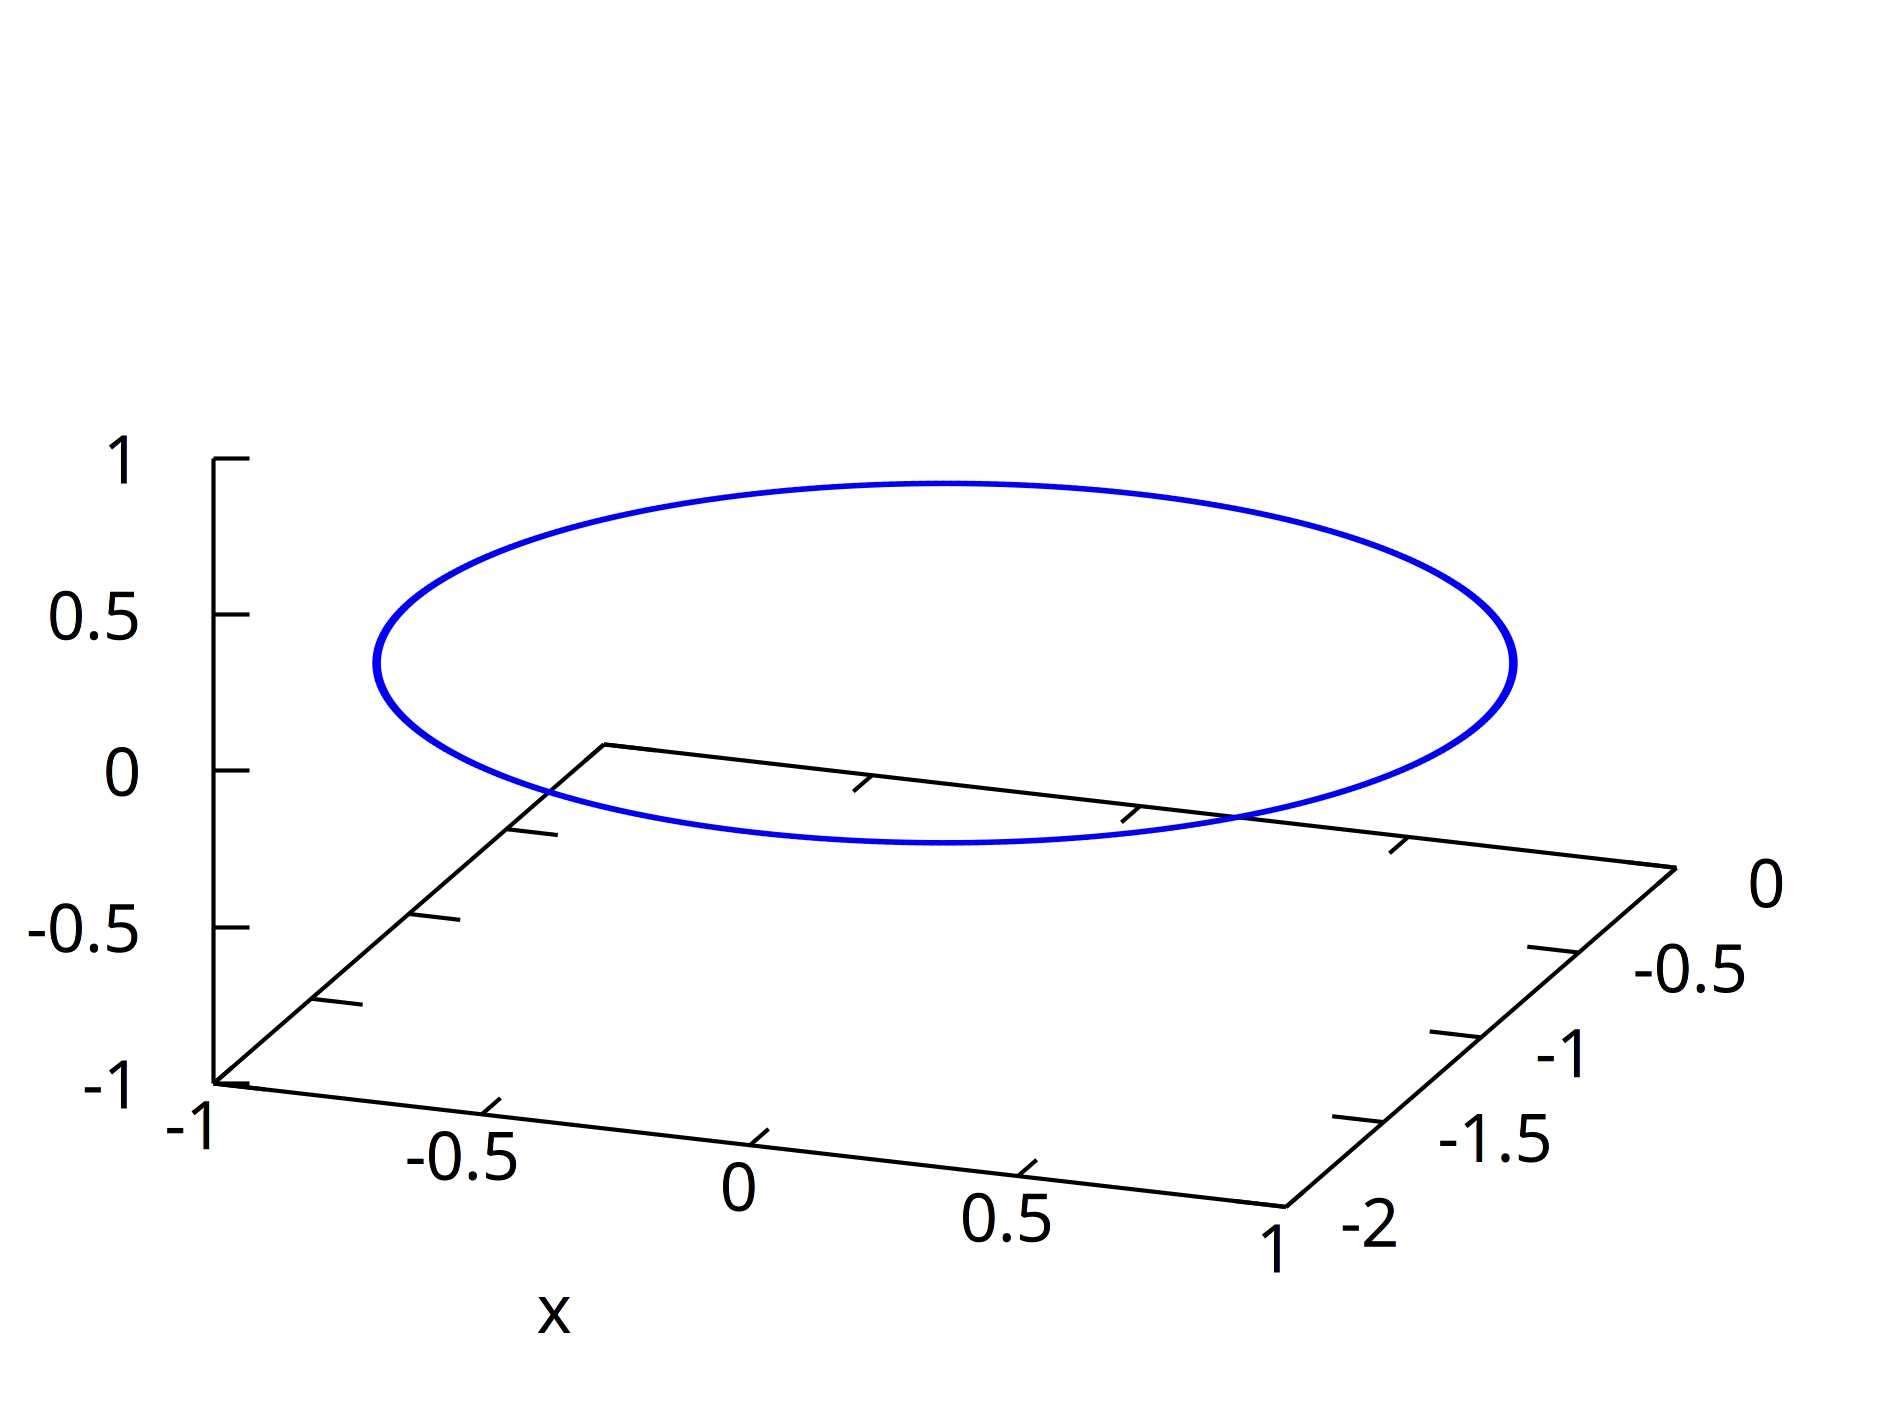
\includegraphics[width=.9\linewidth]{img/3dposizione.png}  
  \caption{Traiettoria della particella}
\end{subfigure}
\begin{subfigure}{.5\textwidth}
  \centering
  % include second image
  \includegraphics[width=.9\linewidth]{img/tempovelocitá.png}  
  \caption{Velocit\`a particella}
\end{subfigure}
\caption{Velocit\`a perpendicolare a $\mathbf{B}$}
\end{figure}


\subsection{Confronto RK2, RK4 e Boris Pusher}
\begin{figure}[ht]
\begin{subfigure}{.5\textwidth}
  \centering
  % include first image
  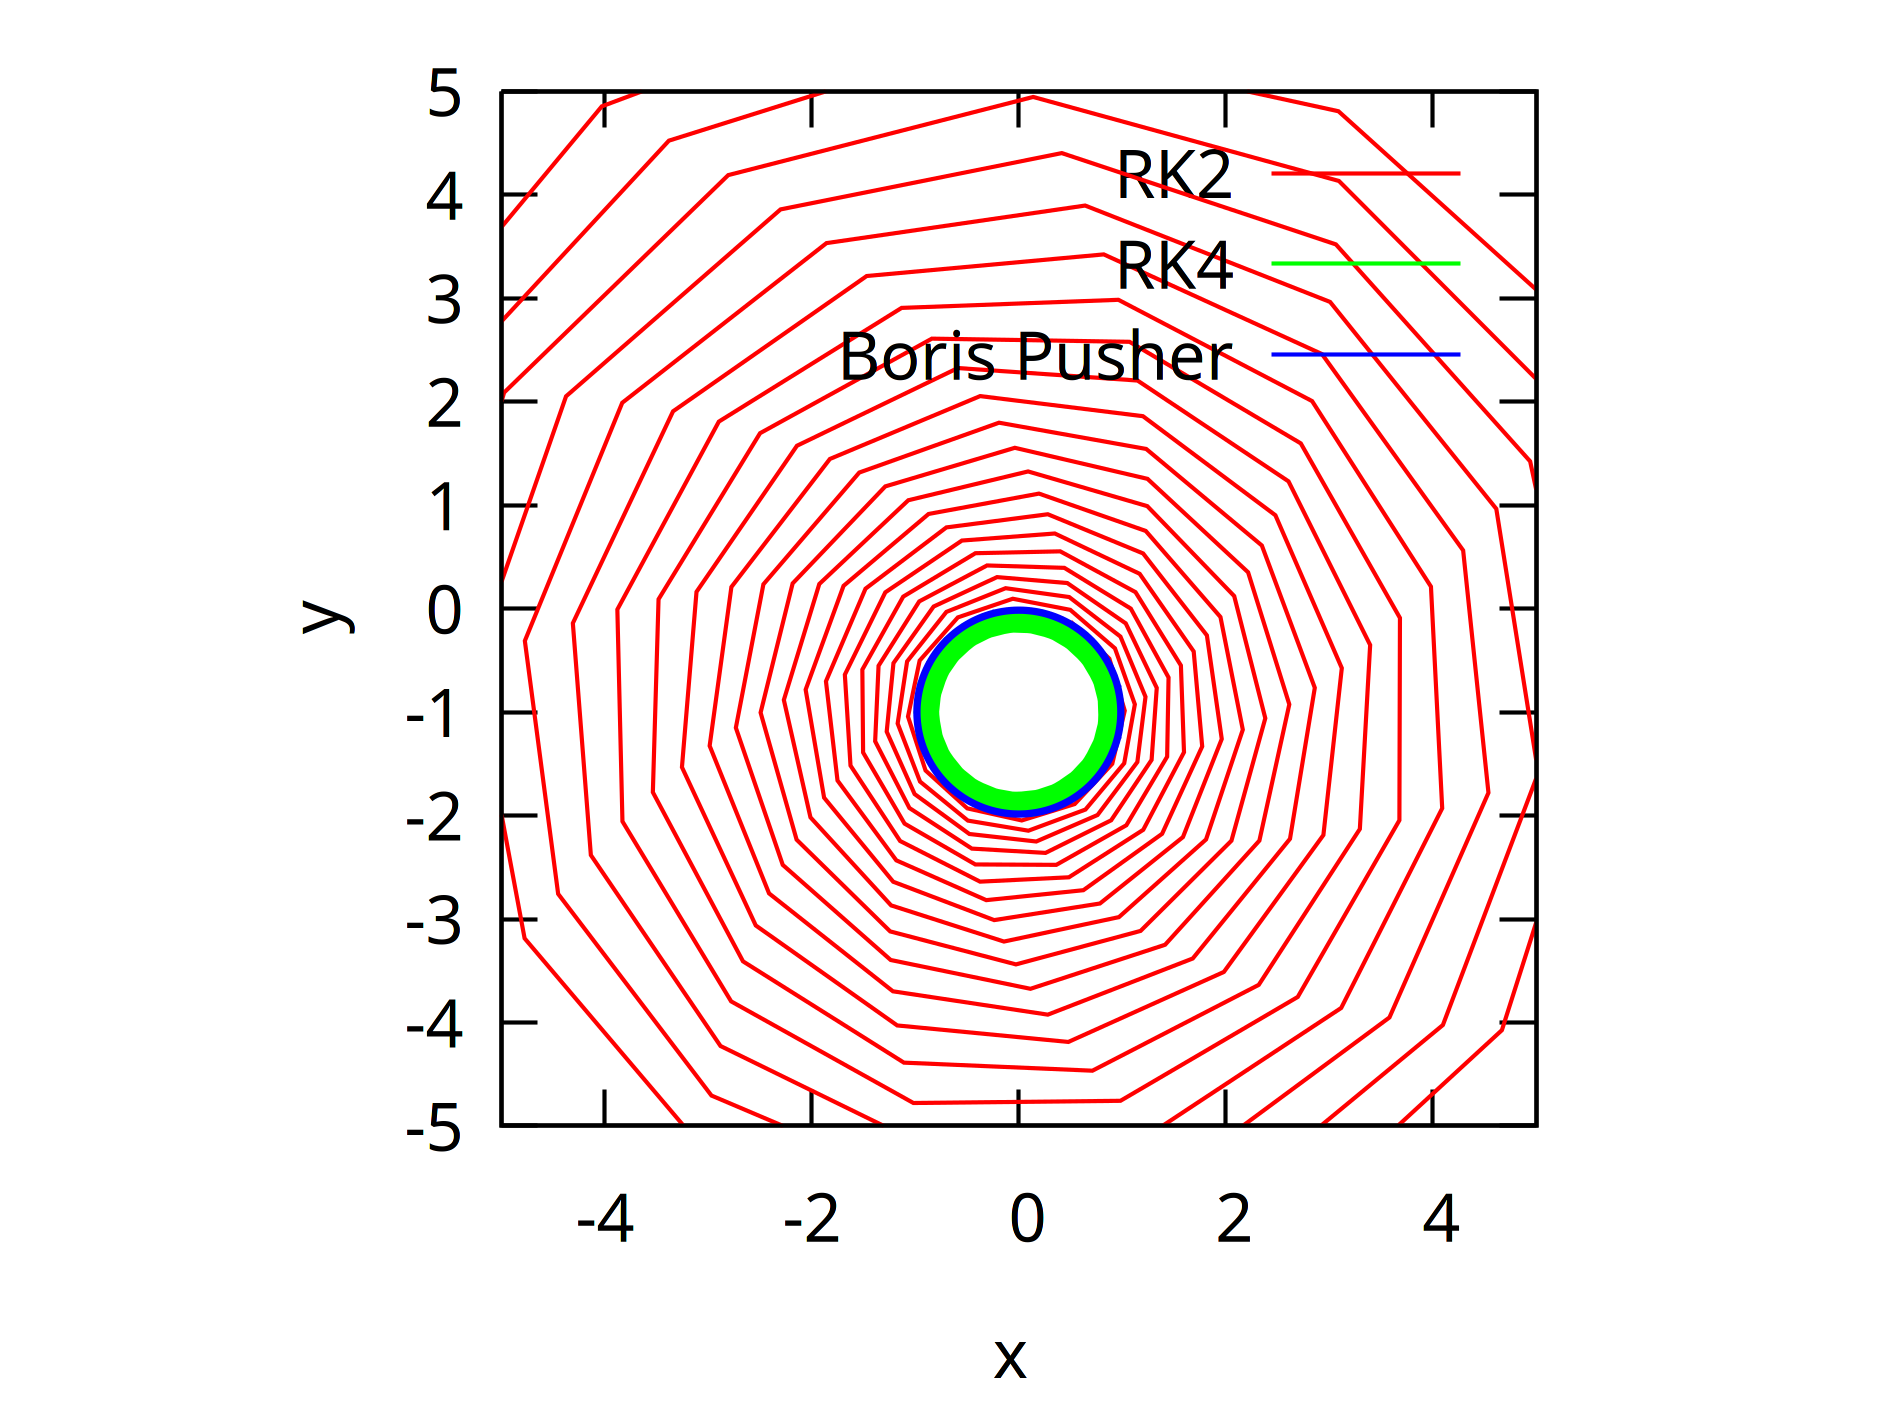
\includegraphics[width=.9\linewidth]{./img/confronto_traiettorie.png}  
  \caption{Confronto tra le traiettorie }
\end{subfigure}
\begin{subfigure}{.5\textwidth}
  \centering
  % include second image
  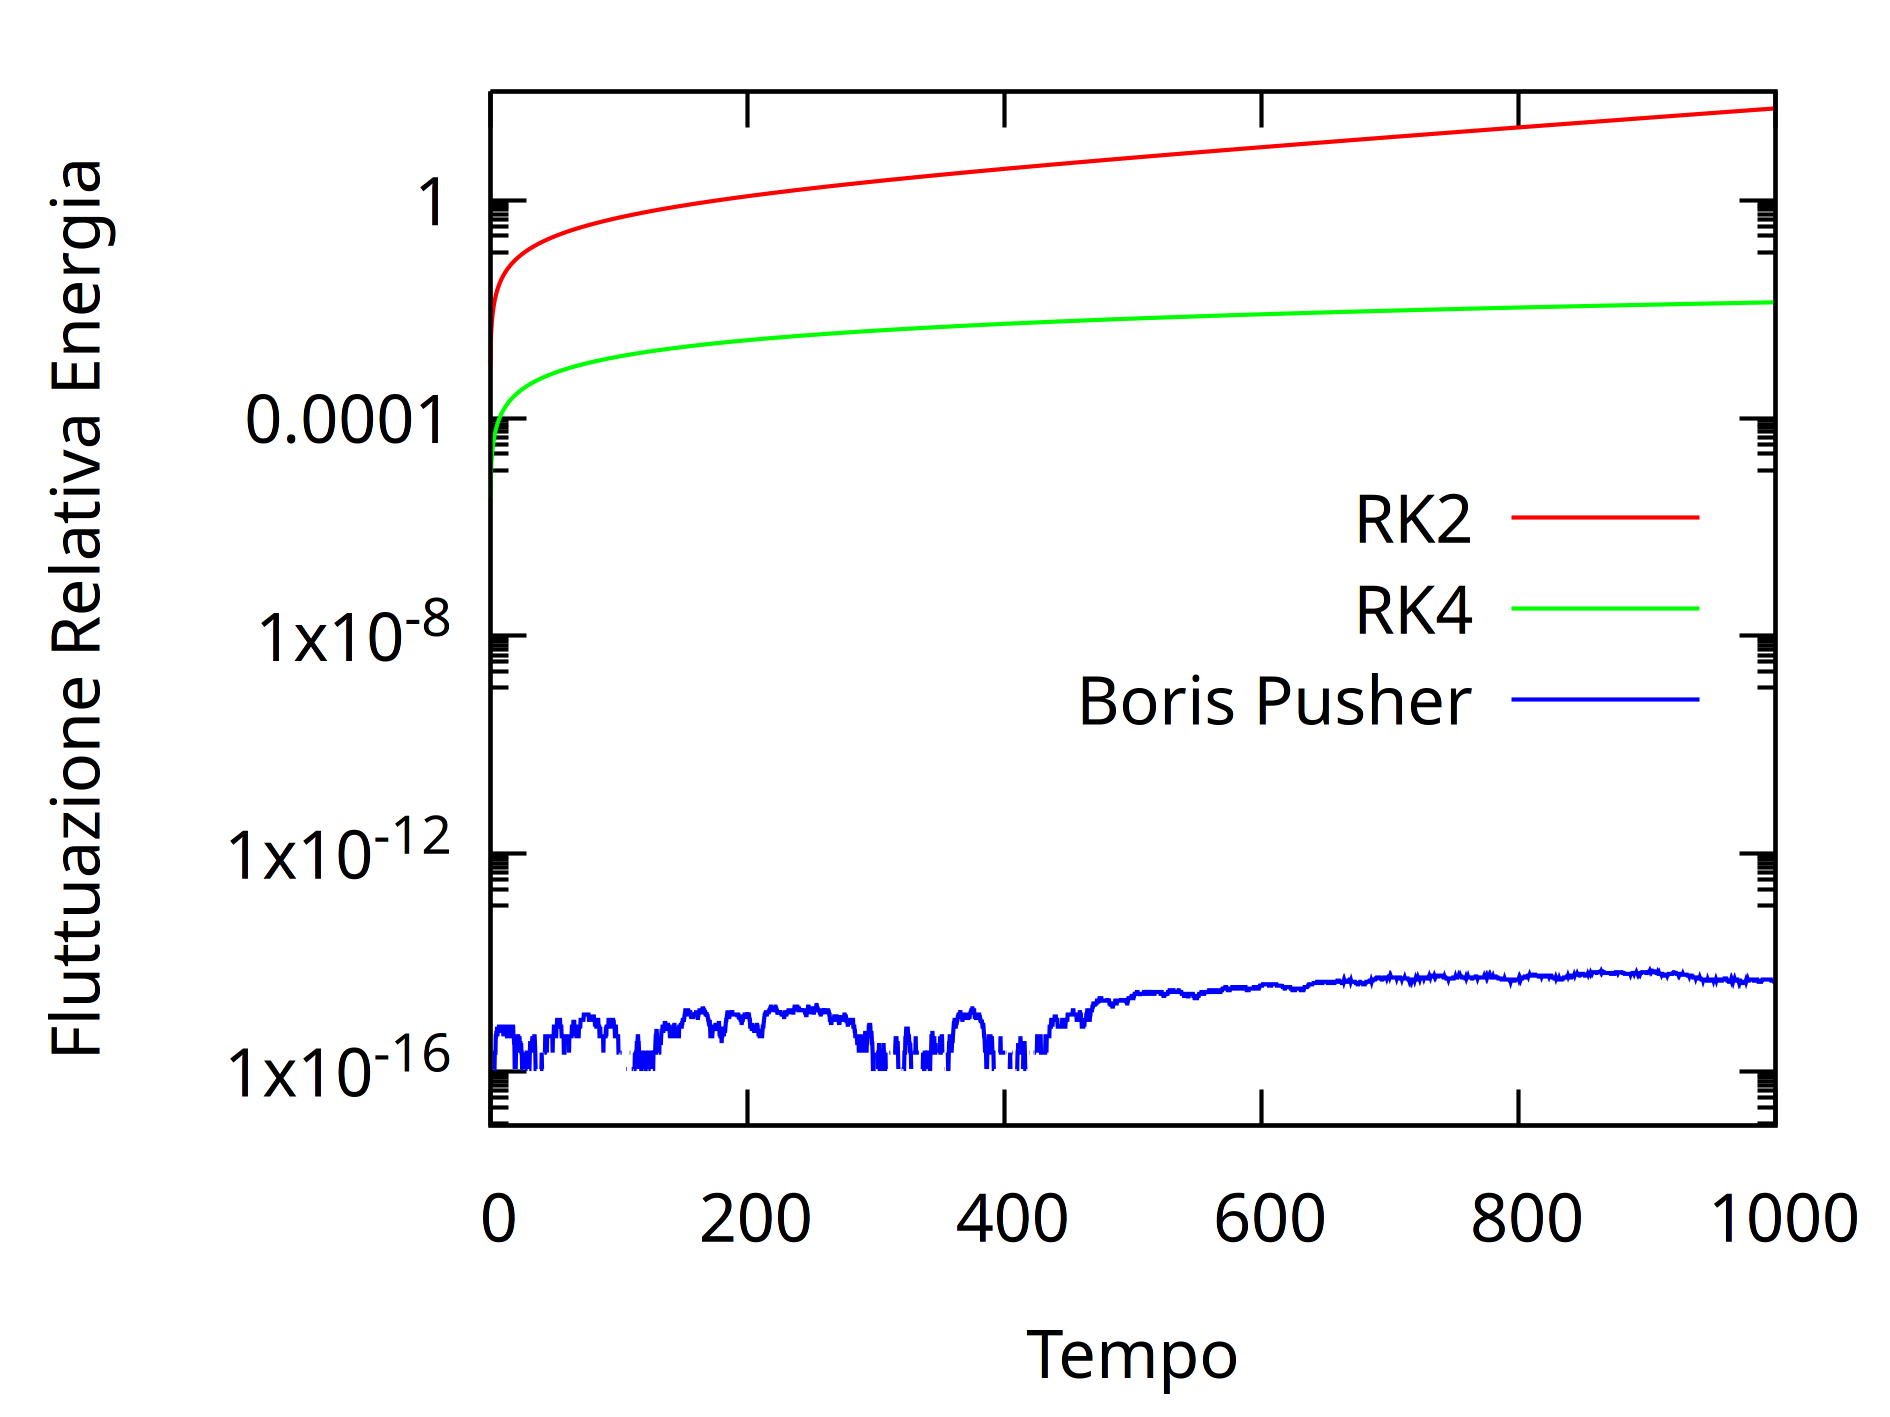
\includegraphics[width=.9\linewidth]{./img/erroreE.png}  
  \caption{Fluttuazione relativa dell'energia totale}
\end{subfigure}
\caption{Confronto tra RK2, RK4 e Boris Pusher con un timestep $\Delta t$= 0.25 e 1000 step}
\end{figure}
Valuto il diverso comportamento dei tre integratori considerando come varia l'energia della particella durante l'integrazione. 
Infatti il sistema fisico considerato conserva l'energia iniziale per cui mi aspetto che anche la simulazione numerica la conservi. \\ 
\begin{equation}\Delta E=\frac{|E-E_0|}{E_0} = \frac{|\mathbf{v}^2 - \mathbf{v}_0^2|}{\mathbf{v}_0^2}\end{equation}
Valuto l'errore relativo sull'energia considerando soltanto l'energia cinetica della particella in quanto il campo magnetico B non fornisce energia in quanto è sempre perpendicolare alla direzione di spostamento, influisce quindi soltanto sulla direzione della velocit\`a e non sul modulo.
L' errore per RK2 e RK4 raggiunge valori rilevanti e continuerebbe a crescere, mentre l'algoritmo di Boris mantiene un errore trascurabile costante compreso tra a $10^{-16}$ e $10^{-14}$. Verifichiamo  che l'uso di un integratore simplettico permette la conservazione dell'energia iniziale.
Nelle simulazioni seguenti sar\`a implementato l'integratore di Boris.


\section{ExB Drift}
\subsection{Soluzione analitica}
Ora consideriamo il moto di una particella in moto in presenza anche di un campo elettrico $\mathbf{E}$ oltre al campo magnetico $\mathbf{B}$. \\ 
\begin{equation}\mathbf{B}=(0,0,B_z)    \end{equation}
\begin{equation}\mathbf{E}=(0,E_y,0)  \end{equation}
Posso scrivere la $\mathbf{v}$ della particella come somma di una componente parallela e una perpendicolare a $\mathbf{B}$: 
$\mathbf{v} = \mathbf{v_{\parallel}} + \mathbf{v_{\perp}}$. \\
A sua volta $\mathbf{v_{\parallel}} = \mathbf{v_d} + \mathbf{v_g}(t)$
assumendo che la velocitá di drift sia costante nel tempo.
L'idea é quella di ricondurci a un moto piú semplice effettuando un cambio di sistema di riferimento.
Infatti, posso riscrivere \eqref{eq:1} come:
\begin{equation}
\frac{d\mathbf{v_g}}{dt} = \mathbf{E} + (\mathbf{v_d} + \mathbf{v_g}) \times \mathbf{B}\end{equation}
\begin{equation}
\frac{d\mathbf{v_g}}{dt} = \left(\mathbf{E} + \mathbf{v_d} \times \mathbf{B}\right) + \mathbf{v_g} \times \mathbf{B}
\end{equation}
Posso annullare il termine con il campo elettrico imponendo una determinata $\mathbf{v_d}$:
\begin{equation}
\mathbf{E} + \mathbf{v_d} \times \mathbf{B} = 0
\end{equation}
Applico il prodotto esterno a entrambi i membri e usando un' identitá vettoriale, ottengo:
\begin{equation}
\mathbf{v_d} = \frac{\mathbf{E} \times \mathbf{B}}{\|\mathbf{B}\|^2}
\end{equation}
Mi sono spostato su un sistema di riferimento il cui campo $\mathbf{E}$ é nullo, per cui ritrovo un semplice moto di girazione:
\begin{equation}
\frac{d\mathbf{v_g}}{dt} = \mathbf{v_g} \times \mathbf{B}
\end{equation}
Se considero $\mathbf{B}=(0,0,B_z)$ e $\mathbf{E}=(0,E_y,0)$ avró:
\begin{equation}
\mathbf{v_d} = \frac{\mathbf{E} \times \mathbf{B}}{\|\mathbf{B}\|^2} = \frac{E_y}{B_z} \vec{i}
\end{equation}  
Posso riscrivere l'equazioni del moto come:
\begin{equation}
\begin{cases} 
\frac{d(v_x - v_d)}{dt}=v_y B_z \\ 
\frac{dv_y}{dt}=-(v_x - v_d)B_z + E_y  \\ 
\frac{dv_z}{dt}=0 
\end{cases}
\end{equation}
La cui soluzione sará:
\begin{equation}
\begin{cases}
v_x = \frac{E_y}{B_z} (1 + \cos(t)) \\
v_y = - \frac{E_y}{B_z}\sin(t) \\
v_z = 0 
\end{cases}
\end{equation}
La traiettoria della particella é una cicloide lungo la direzione x. Il moto è inaspettato avendo un campo elettrico agente lungo $y$, infatti ci aspetteremmo che la particella accelleri lungo questa direzione.\\
In realt\`a, quando la velocit\`a della particella aumenta cresce anche la forza risultante dall'interazione con $\mathbf{B}$, sempre normale alla traiettoria.
Infatti la carica ferma nell'origine subisce un accelerazione lungo y dovuta a $\mathbf{E}$. Appena la carica inizia a muoversi la forza magnetica agisce nella direzione normale alla traiettoria. Questo fino alla fine del periodo dove la forza risultante è nulla, per cui la carica si ferma e il moto si ripete periodico.\\


\subsection{Convergenza degli integratori}

Nel caso precedente di girazione abbiamo studiato le proprietá di conservazione dell'energia dei tre integratori, ora vorremmo studiarne le proprietá di convergenza.
Per fare ció confronteró la soluzione analitica trovata nella sezione precedente con la soluzione numerica. Questo verrá ripetuto per differenti timestep $\Delta t$.
Come valori per $\mathbf{E}$, $\mathbf{B}$ e $\mathbf{v_0}$ della particella useremo:
\begin{equation}\mathbf{B}=(0,0,1) \end{equation}
\begin{equation}\mathbf{E}=(0,\frac{1}{2},0) \end{equation}
\begin{equation}\mathbf{v_0} = (1,0,0)\end{equation}
\begin{figure}[ht]
  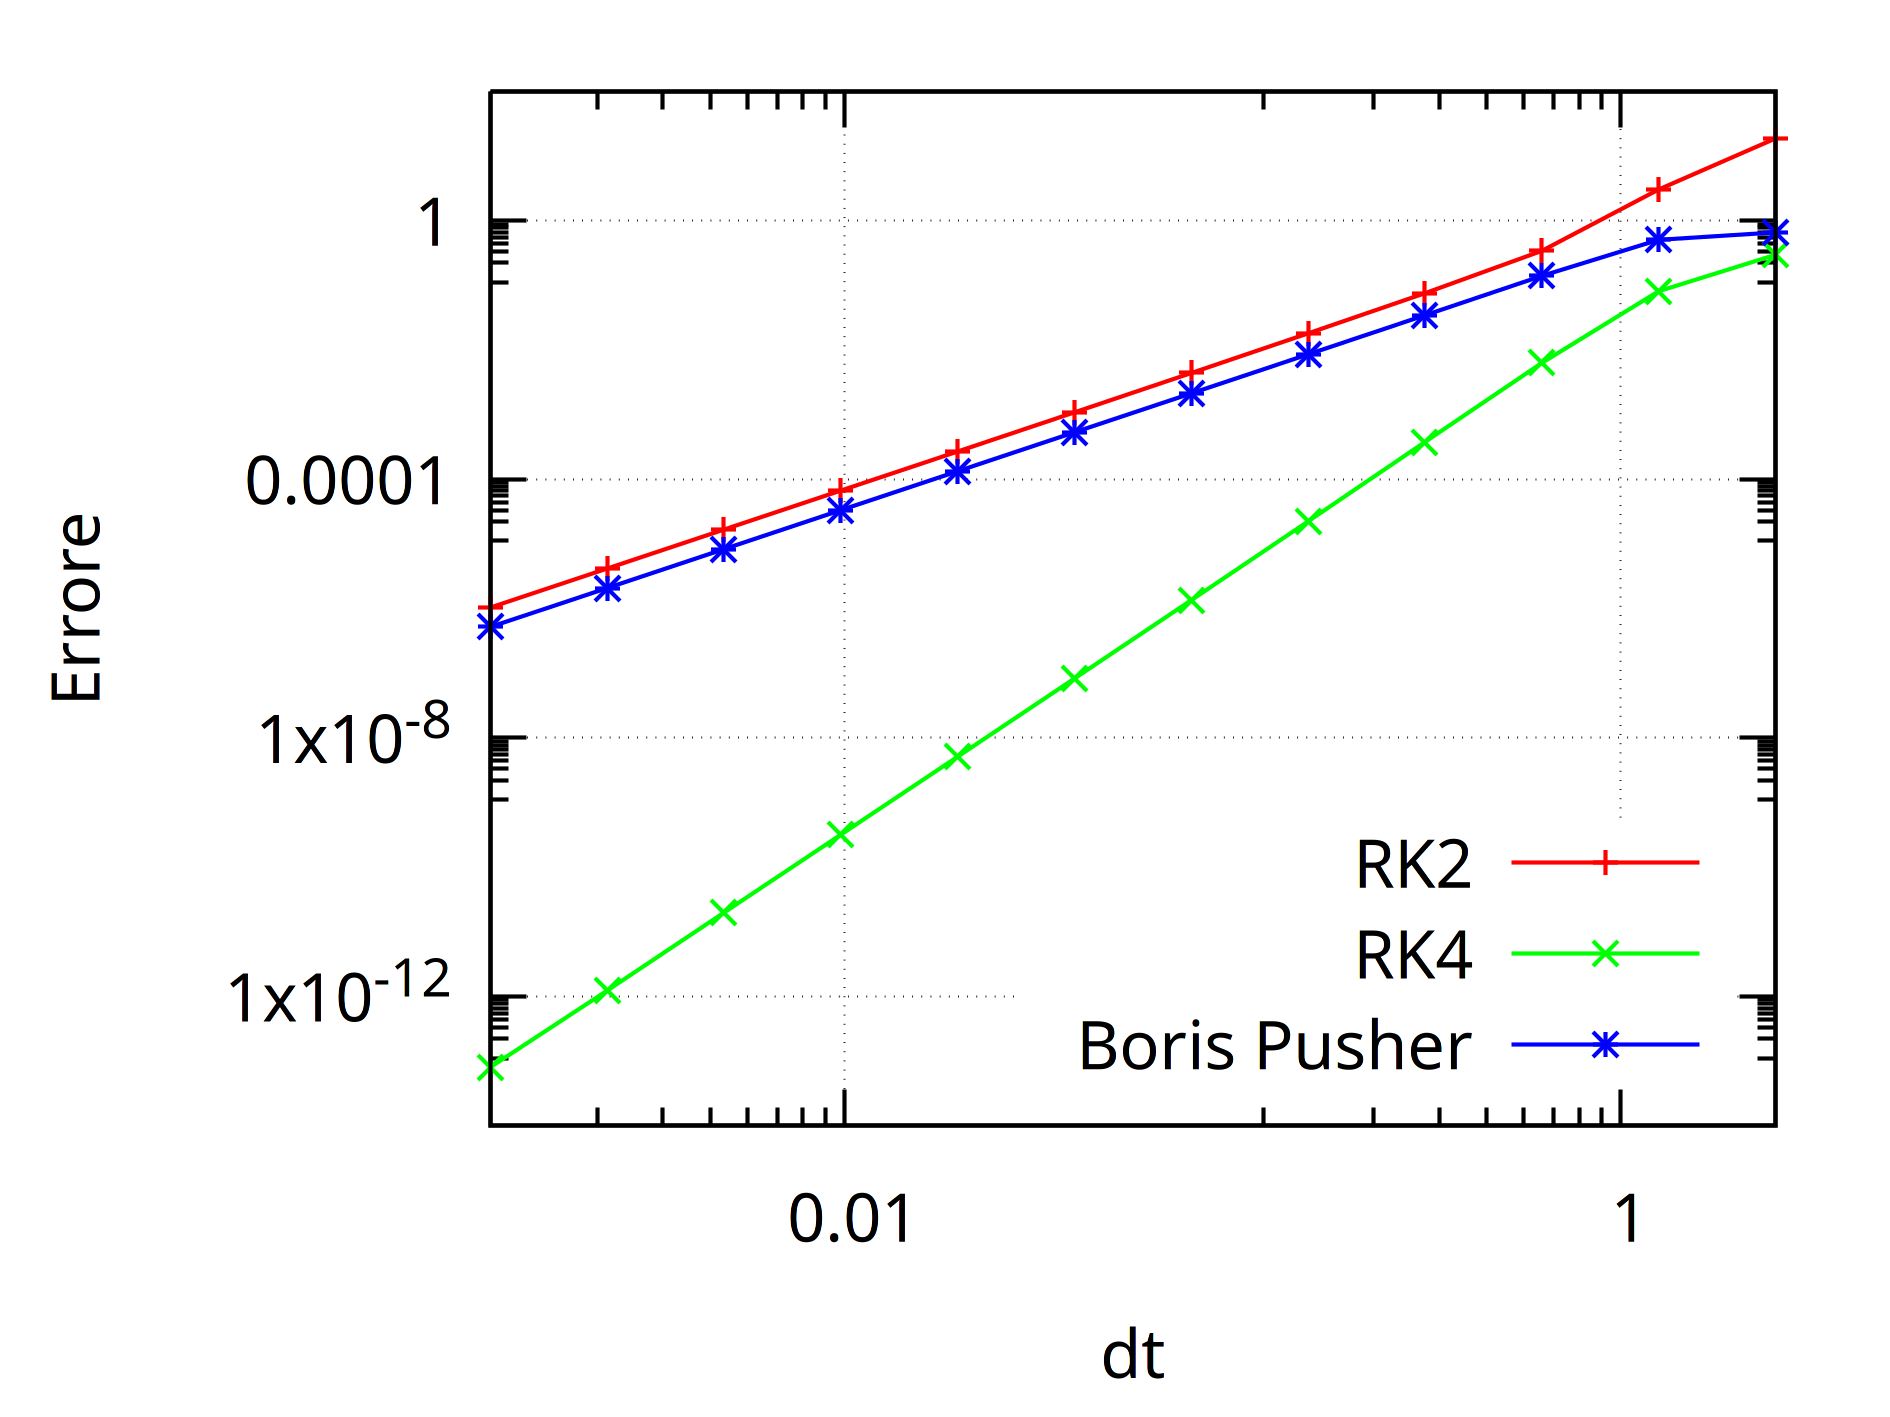
\includegraphics[width=.9\linewidth]{img/convergenza.png}  
  \caption{Errore al variare del timestep $\Delta t$}
\end{figure}%

Verifichiamo come RK2 e Boris Pusher siano integratori del $2^o$ ordine: un fattore 10 per $\Delta t$ comporta una riduzione di 100 nell'errore. RK4 é del $4^o$ ordine per cui a un fattore 10 del $\Delta t$ corrisponde una riduzione di $10^4$ per l'errore.

\newpage
\subsection{Soluzione Numerica}
Come integratore usiamo Boris Pusher,in quanto nonostante una minore precisione rispetto a RK4 otteniamo un' accuratezza sufficiente: $10^{-4}$ con timestep $\Delta t = 10^{-2}$.\\
Come valori per $\mathbf{E}$, $\mathbf{B}$ e $\mathbf{v_0}$ della particella useremo:
\begin{equation}\mathbf{B}=(0,0,1) \end{equation}
\begin{equation}\mathbf{E}=(0,\frac{1}{2},0) \end{equation}
\begin{equation}\mathbf{v_0} = (1,0,0)\end{equation}
\begin{figure}[ht]
\begin{subfigure}{.5\textwidth}
  \centering
  % include first image
  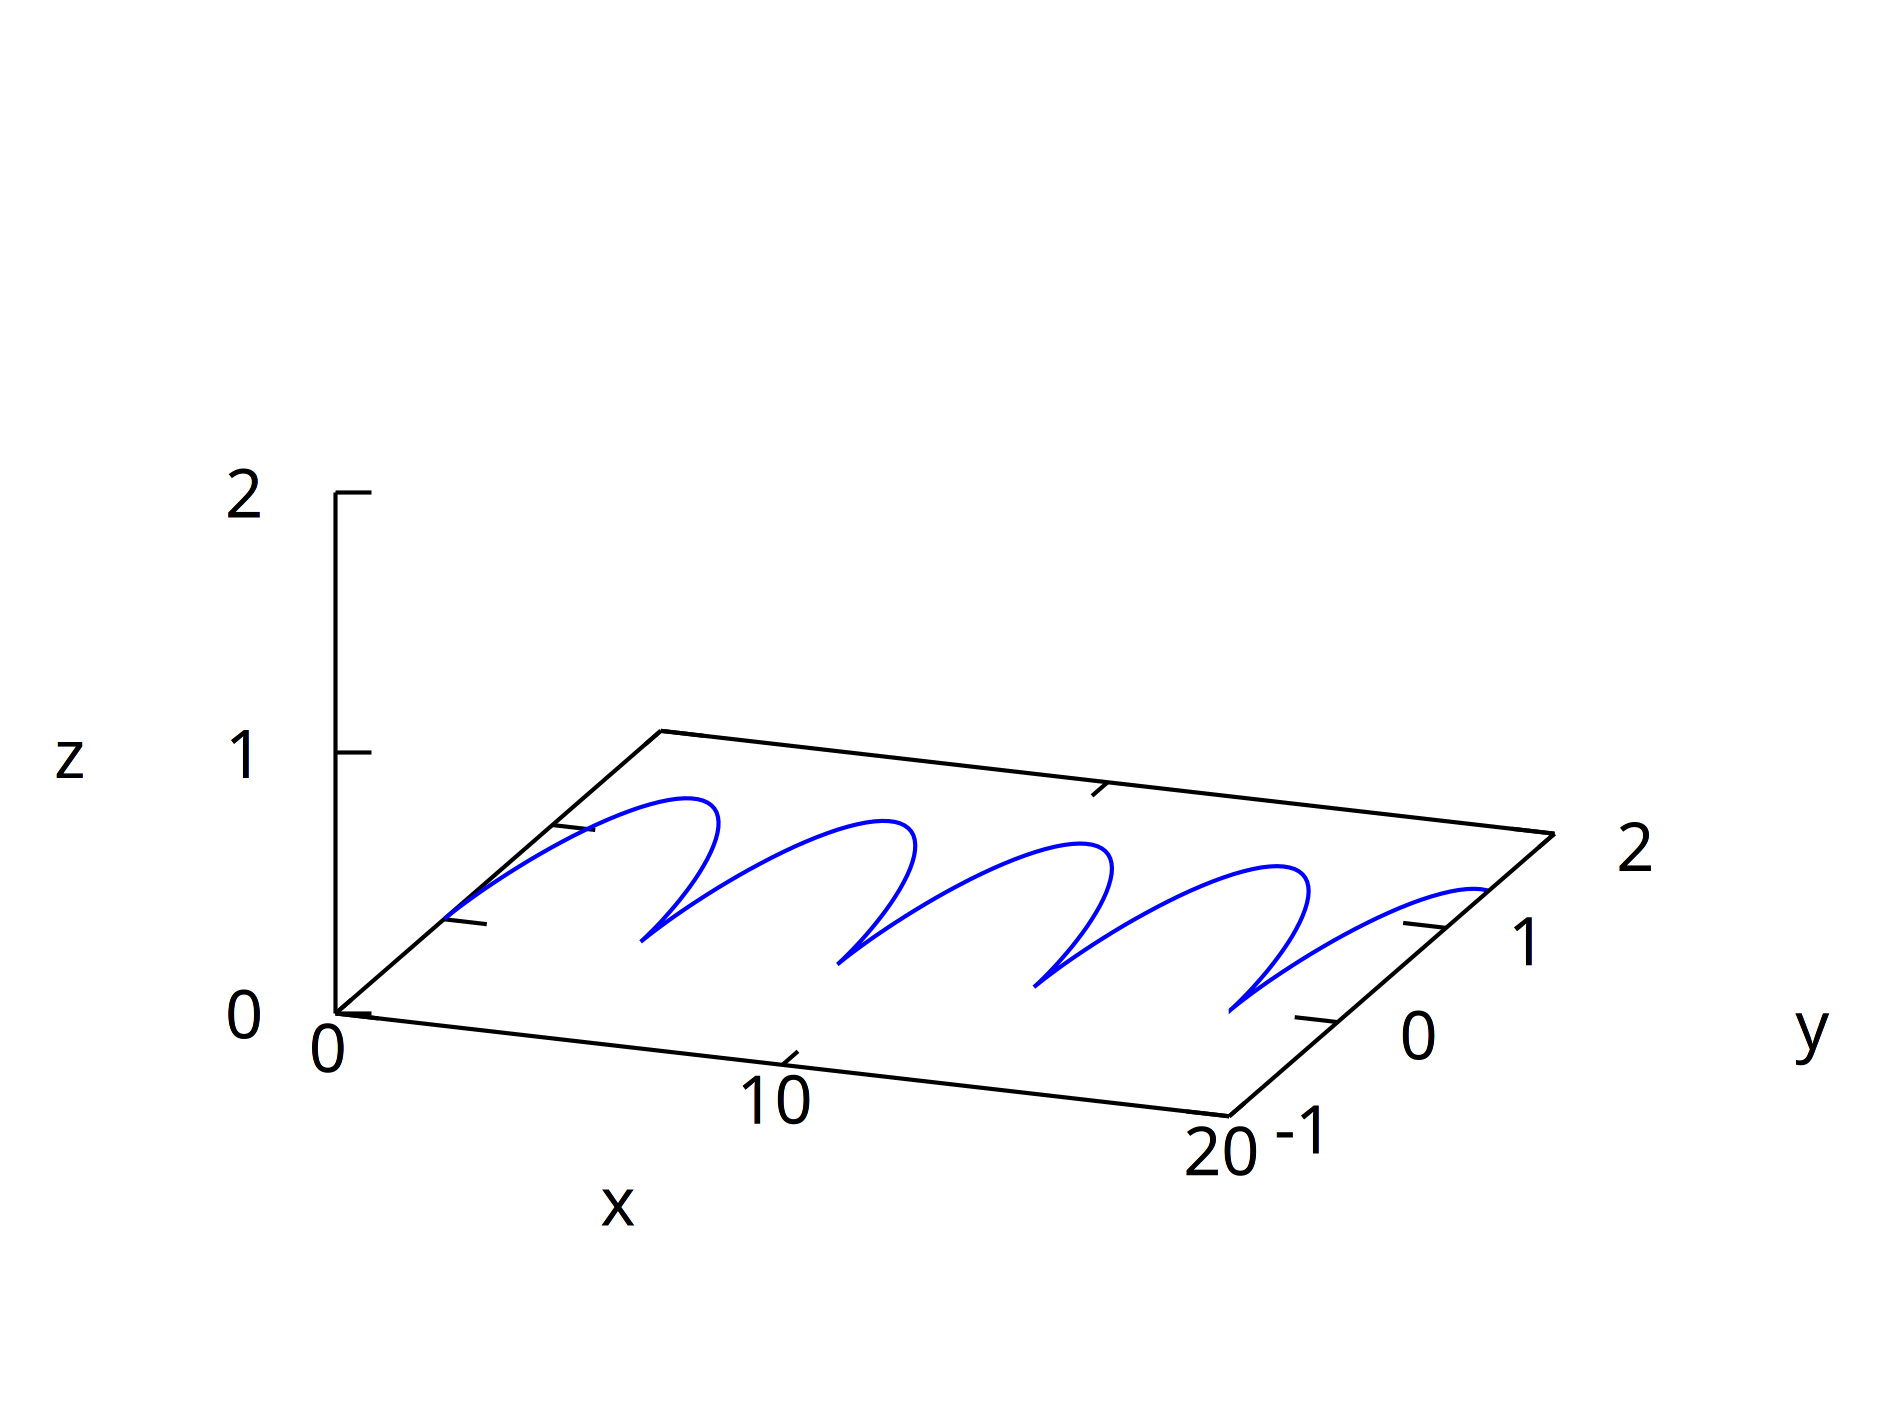
\includegraphics[width=.9\linewidth]{img/3dposizionedrift.png}  
  \caption{Traiettoria nello spazio 3d}
\end{subfigure}
\begin{subfigure}{.5\textwidth}
  \centering
  % include second image
  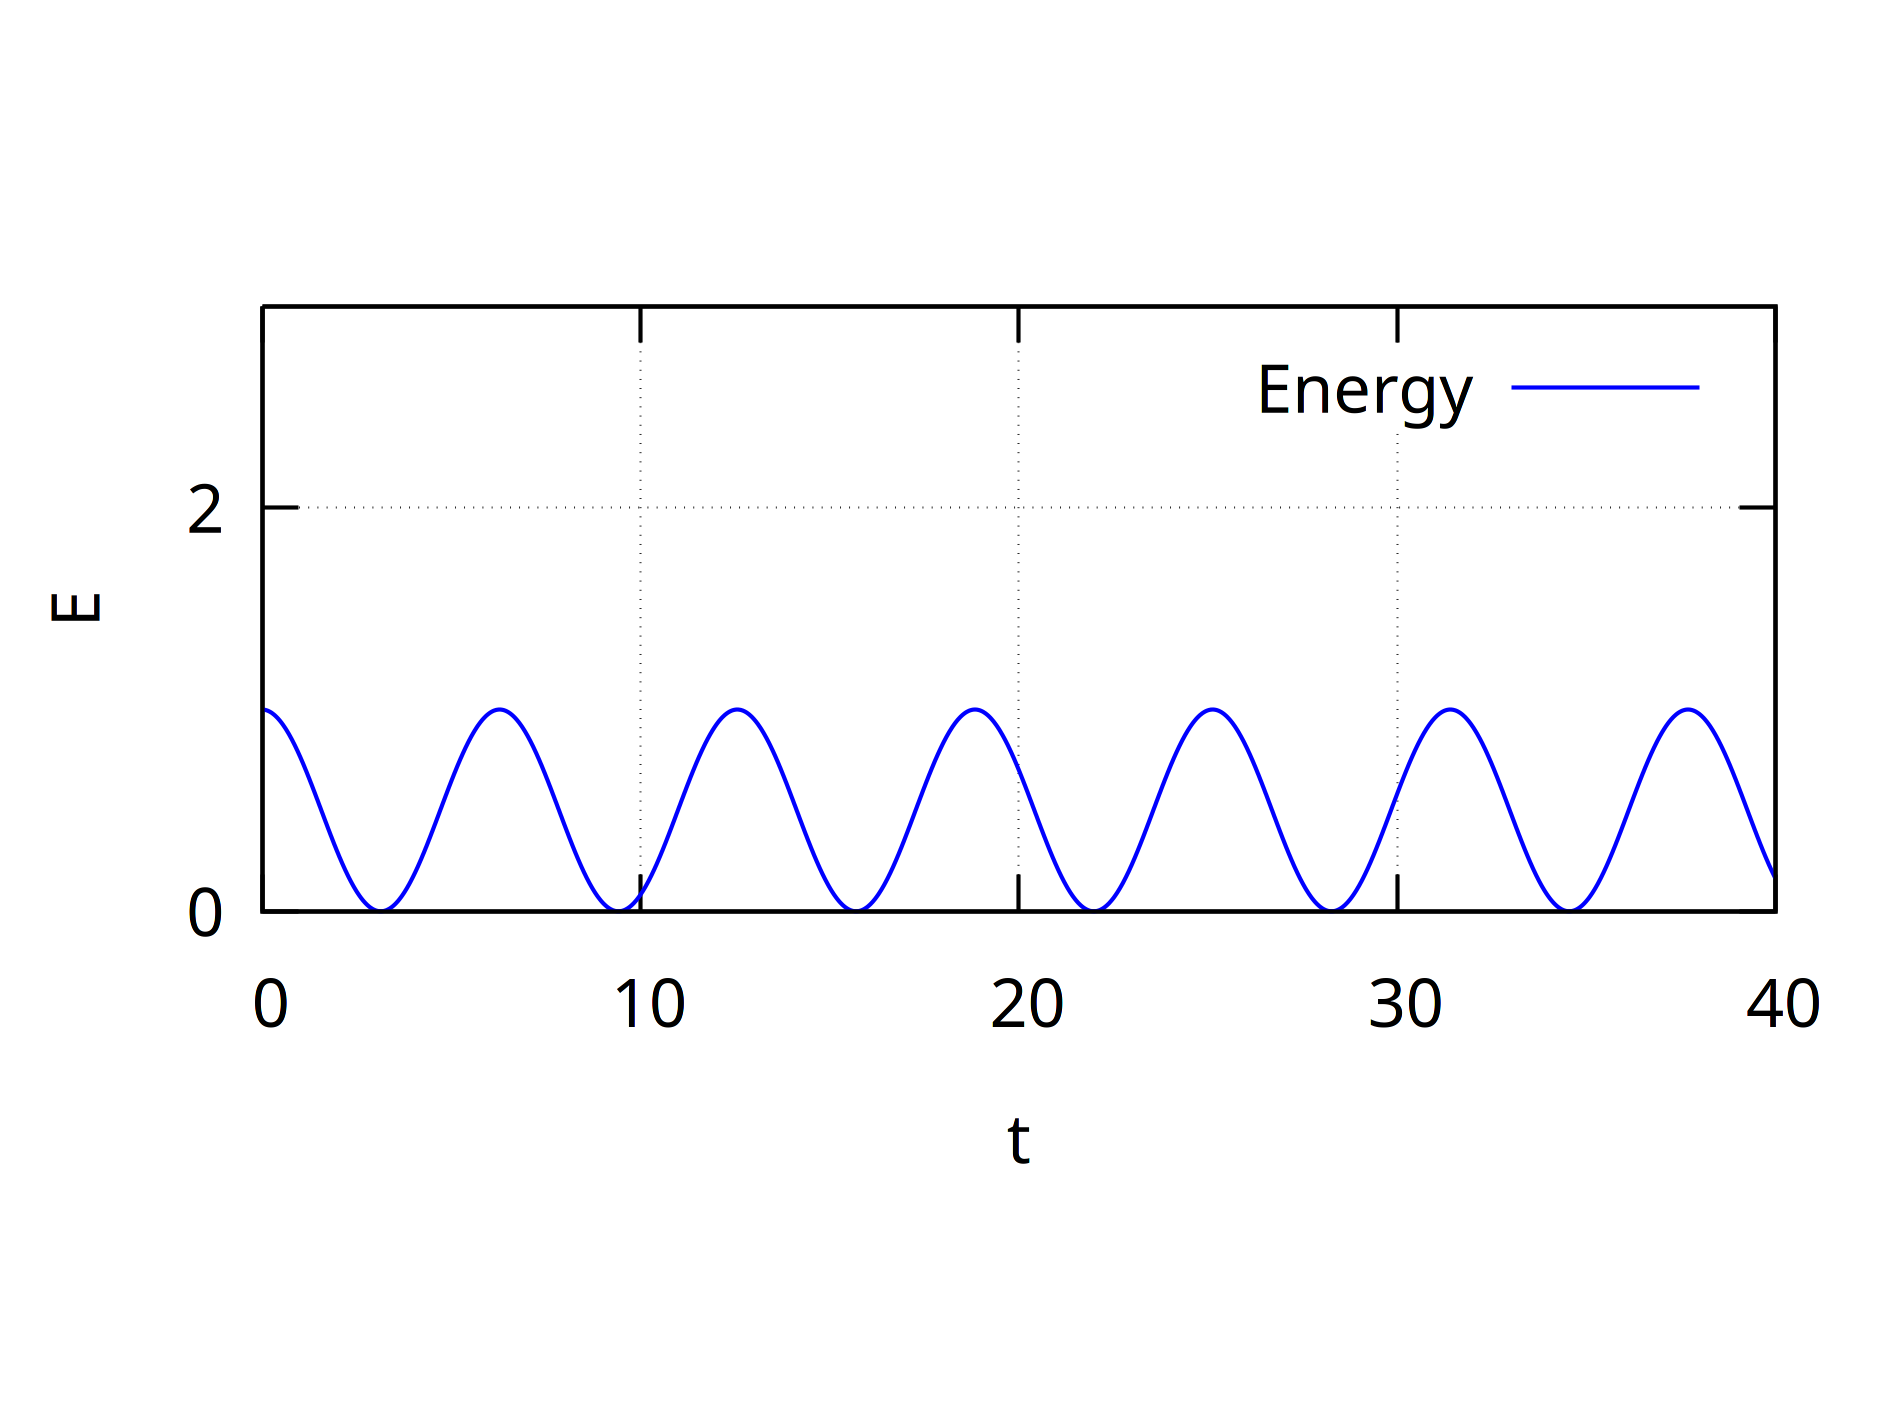
\includegraphics[width=.9\linewidth]{img/energia.png}  
  \caption{Energia}
\end{subfigure}
\caption{ExB Drift}
\end{figure}%
Si puó notare come la particella non abbia un guadagno netto di energia cinetica. Lo possiamo spiegare grazie alla derivazione della sezione precedente: se ci spostiamo in un sistema di riferimento che si muove con $\mathbf{v_d}$ annulliamo il campo $\mathbf{E}$, per cui la particella interagisce soltanto con $\mathbf{B}$. $\mathbf{B}$ non compie lavoro sulla particella, infatti non modifica il modulo della velocitá ma soltanto la direzione. \\
Per essere piú precisi questo cambio di sistema di riferimento puó essere effettuato soltanto se l'invariante relativistico $E^2 - B^2 $ é conservato, per cui $ \|\mathbf{E}\| < \|\mathbf{B}\|$. \\
Se $ \|\mathbf{E}\| > \|\mathbf{B}\|$ l'invariante non é piú conservato e non posso effettuare questo cambio di sistema di riferimento.


\section{Particelle in prossimit\`a di un punto a X}
Posiziono $N = 10^4 $ particelle in un quadrato $L \times L$ con posizione e velocit\`a uniformemente distribuite. In particolare la velocit\`a di ognuna sar\`a $|v|=0.1$ e direzione casuale ottenuta con un angolo casuale tra $0$ e $2\pi$.\\
Le particelle sono immerse in un campo elettrico e magnetico:
\begin{equation}\vec{E}=\left(0,0,\frac{1}{2} \right)\end{equation}
\begin{equation}\vec{B}=\left(\frac{y}{L},\frac{x}{L},0\right) \end{equation} 
Scrivo le equazioni del moto:
\begin{equation}
\begin{cases} 
\frac{dv_x}{dt}= 0 \\ 
\frac{dv_y}{dt}= 0 \\ 
\frac{dv_z}{dt}= \frac{1}{2} + \frac{x}{L}v_x - \frac{y}{L}v_y 
\end{cases}
\end{equation}
Le particelle compiono un moto peculiare, infatti le particelle che si trovano nella zona centrale del quadrato, vengono accellerate maggiormente verso $z$ dando effetto a una sorta di getto di particelle.\\
Verifichiamo per quali particelle nel nostro dominio é possibile cambiare sistema di riferimento:
\begin{equation} \|\mathbf{E}\| < \|\mathbf{B}\|\end{equation}
\begin{equation}\frac{1}{2} < \sqrt{\frac{x^2}{L^2} + \frac{y^2}{L^2}} \end{equation}
\begin{equation} x^2 + y^2 > \frac{L^2}{4}\end{equation}
per cui per le particelle esterne alla circonferenza di raggio $R = \frac{L}{2}$ é possibile annullare il campo $\mathbf{E}$ e non subiranno accelerazione. Mentre le particelle interne subiranno un accelerazione verso $z$.


\begin{figure}
\centering
\begin{subfigure}{0.33\textwidth}
    \centering
    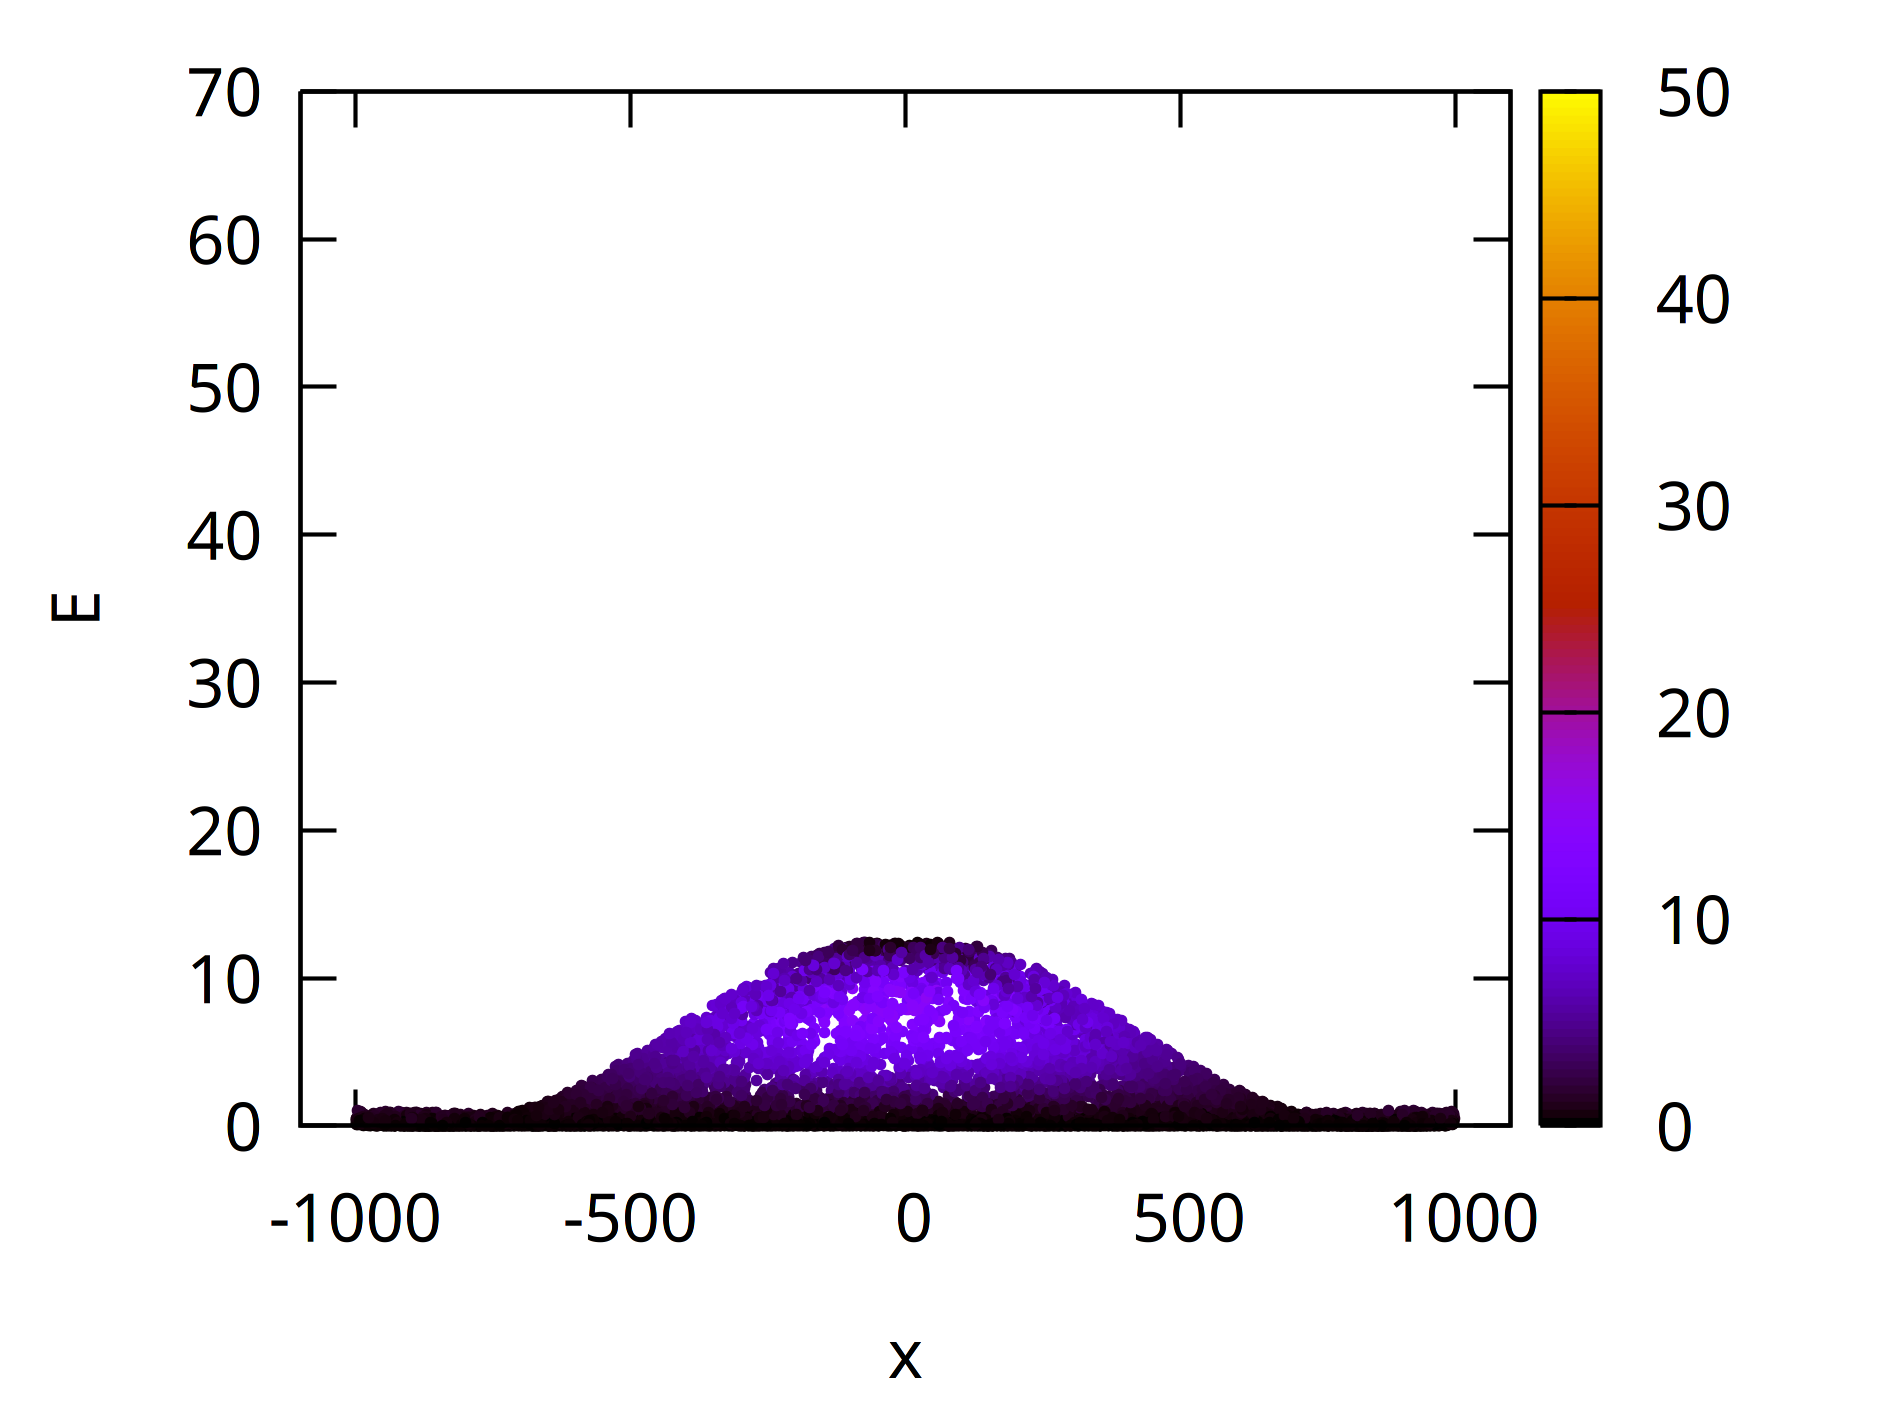
\includegraphics[width=1.\textwidth]{img/energy_70.png}
    \subcaption{t = 7 }
\end{subfigure}%
\begin{subfigure}{0.33\textwidth}
    \centering
    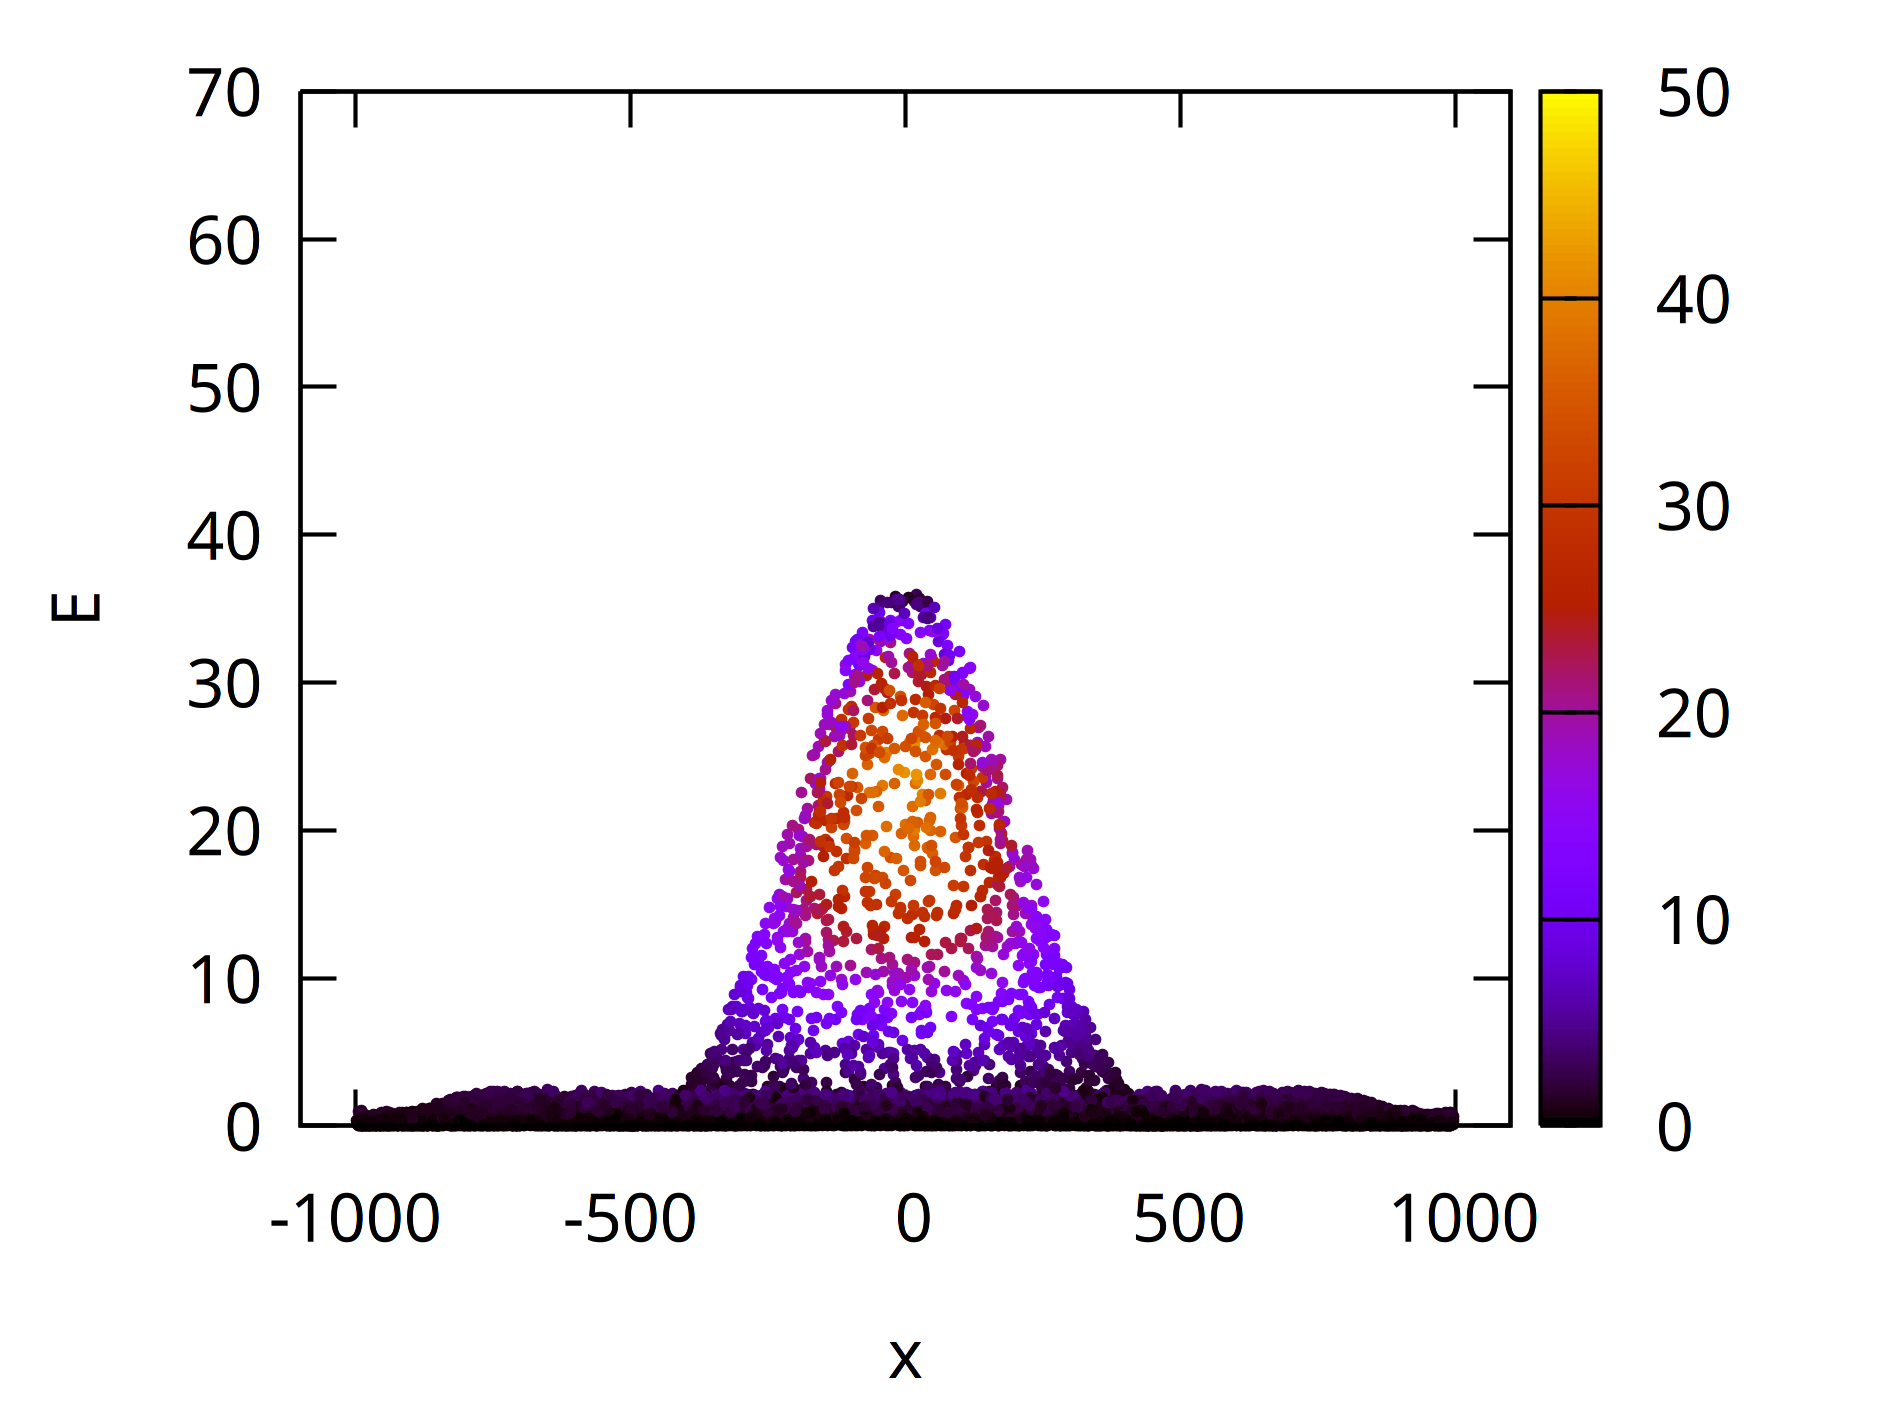
\includegraphics[width=1.\textwidth]{img/energy_120.png}
    \subcaption{t = 12 }

\end{subfigure}%
\begin{subfigure}{0.33\textwidth}
    \centering
    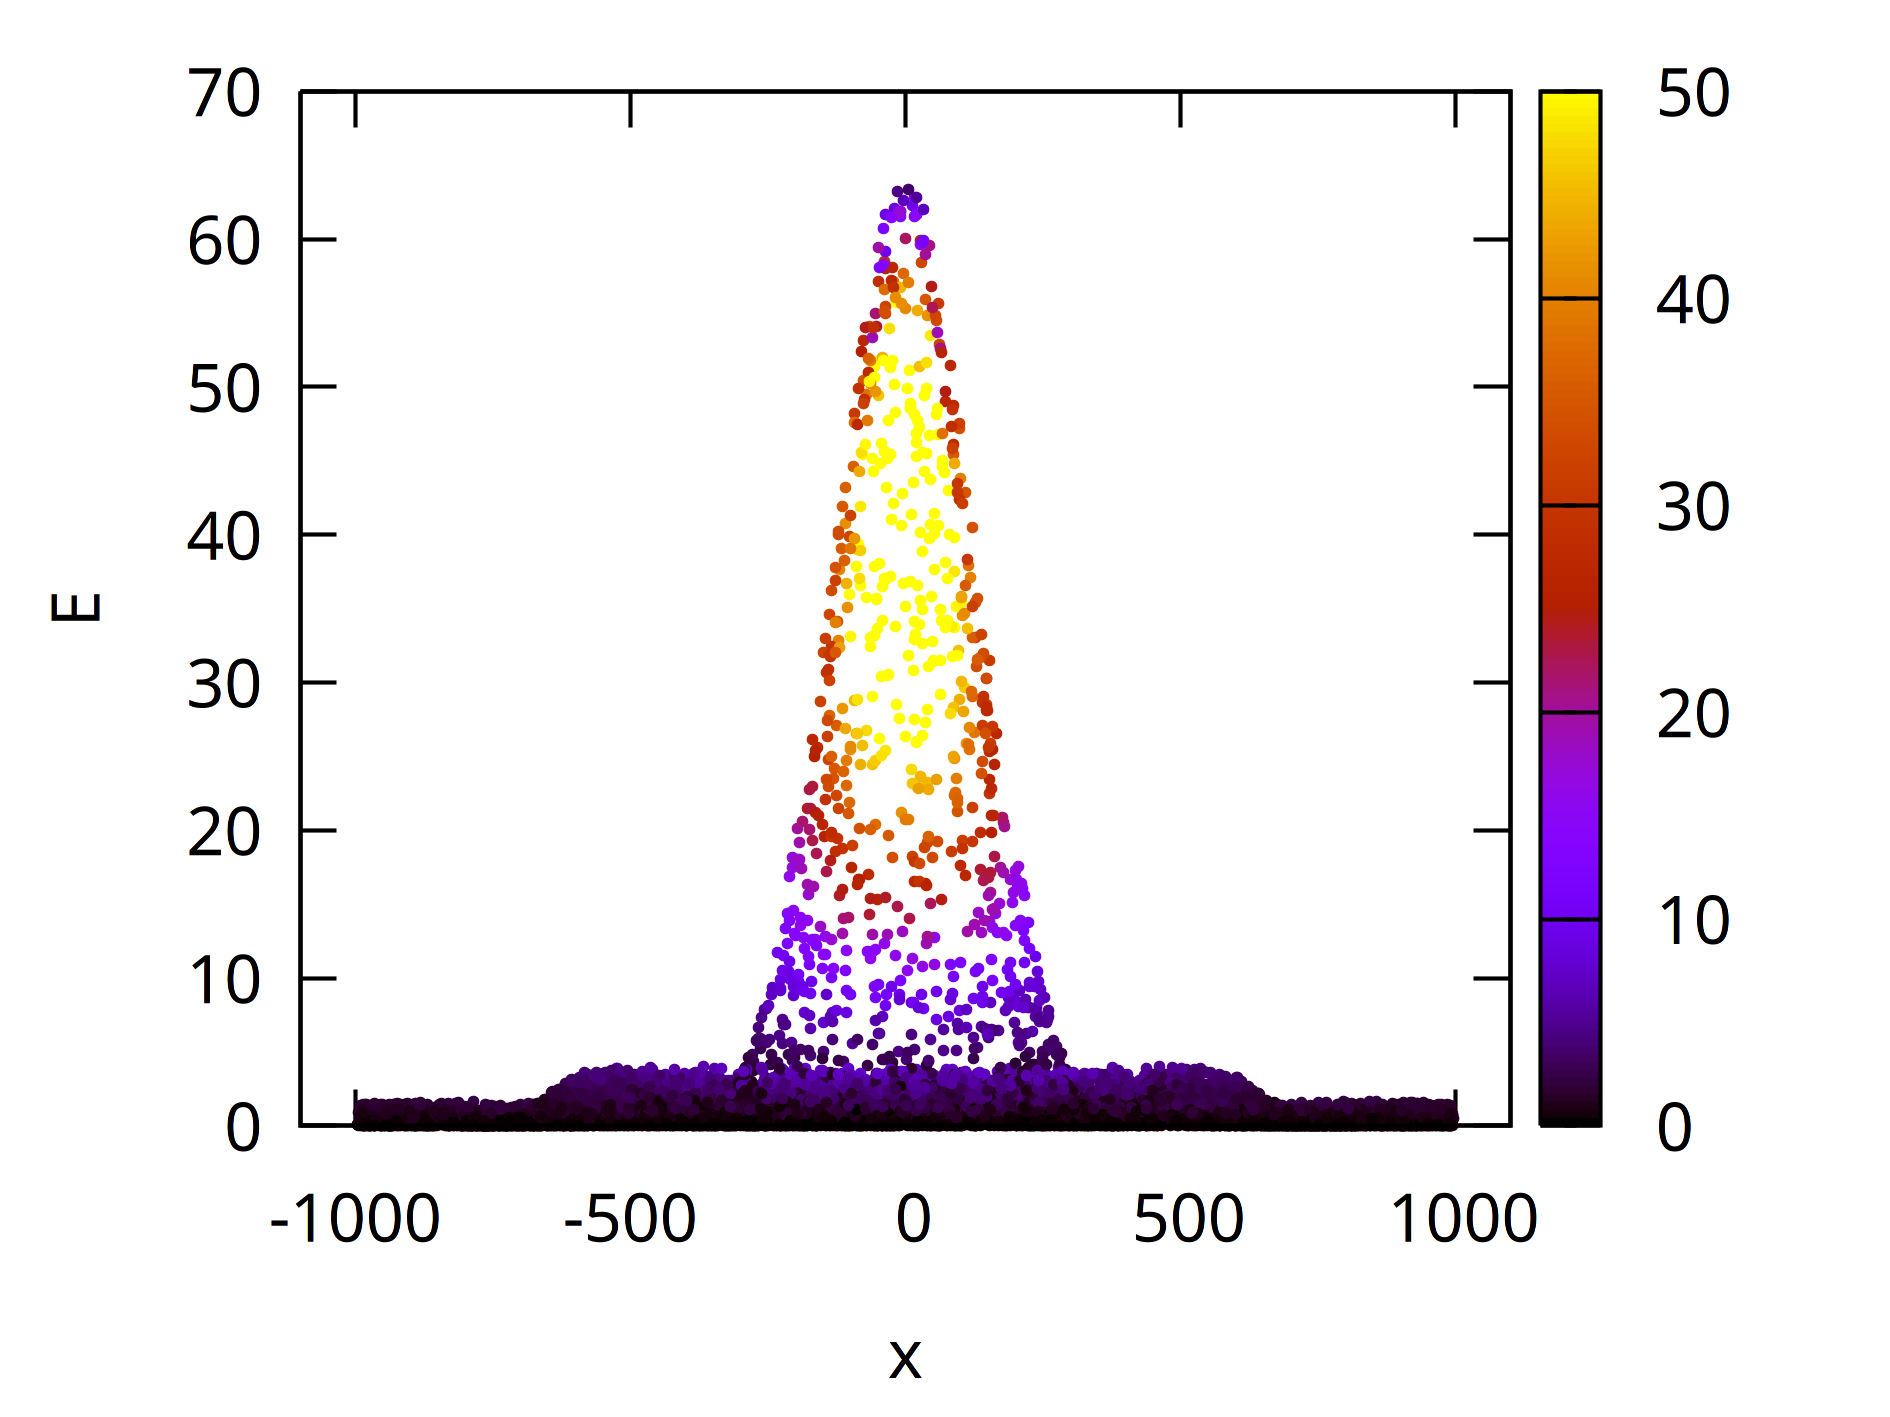
\includegraphics[width=1.\textwidth]{img/energy_160.png}
    \subcaption{t = 16 }
\end{subfigure}



\begin{subfigure}{0.33\textwidth}
    \centering
    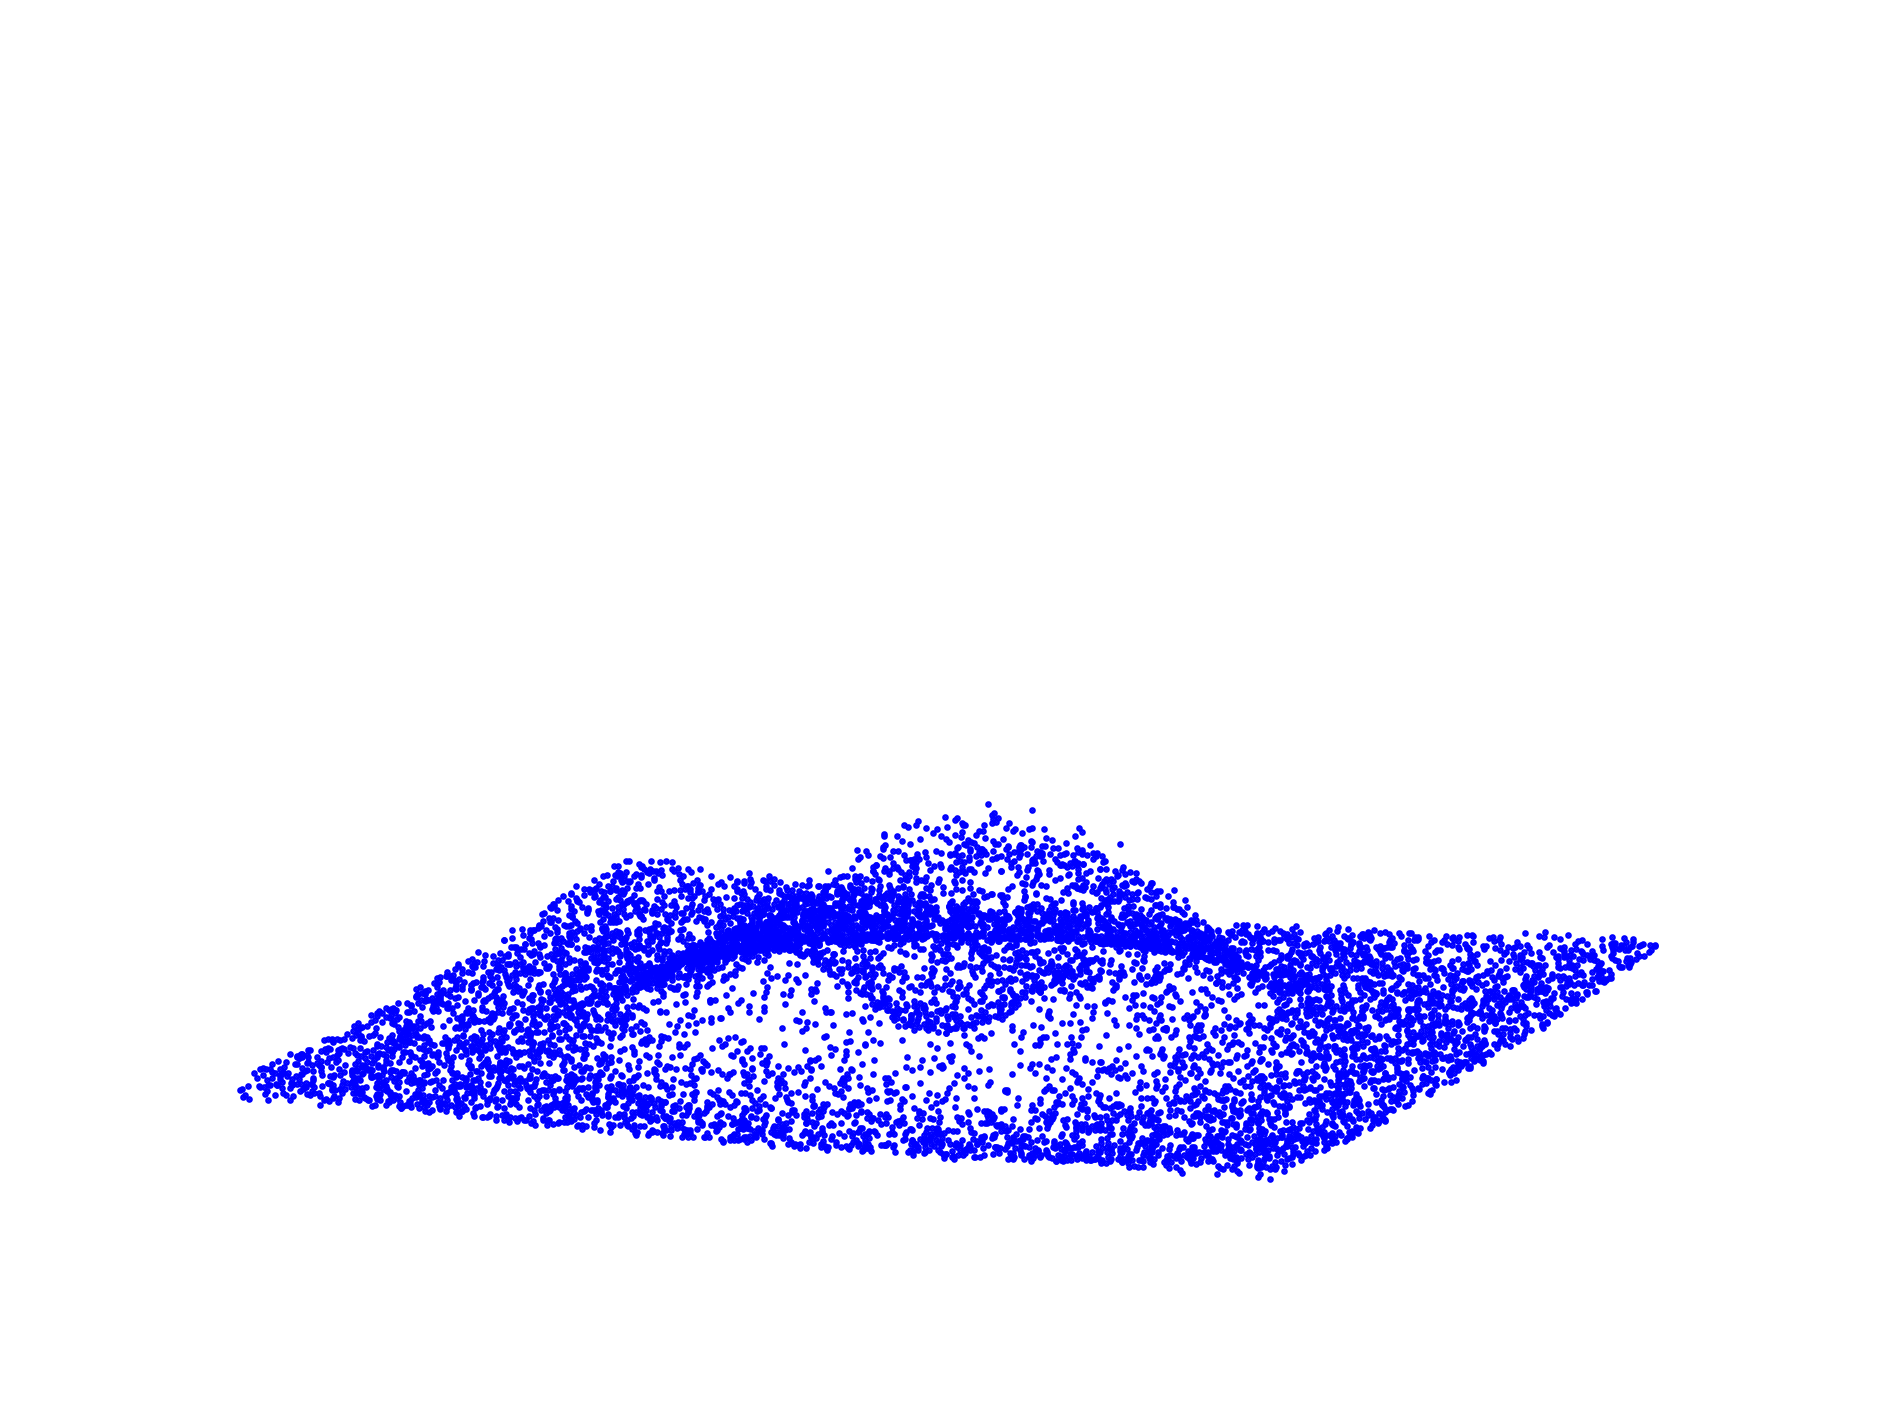
\includegraphics[width=1.\textwidth]{img/distrib_70.png}
    \subcaption{t = 70 }
\end{subfigure}%
\begin{subfigure}{0.33\textwidth}
    \centering
    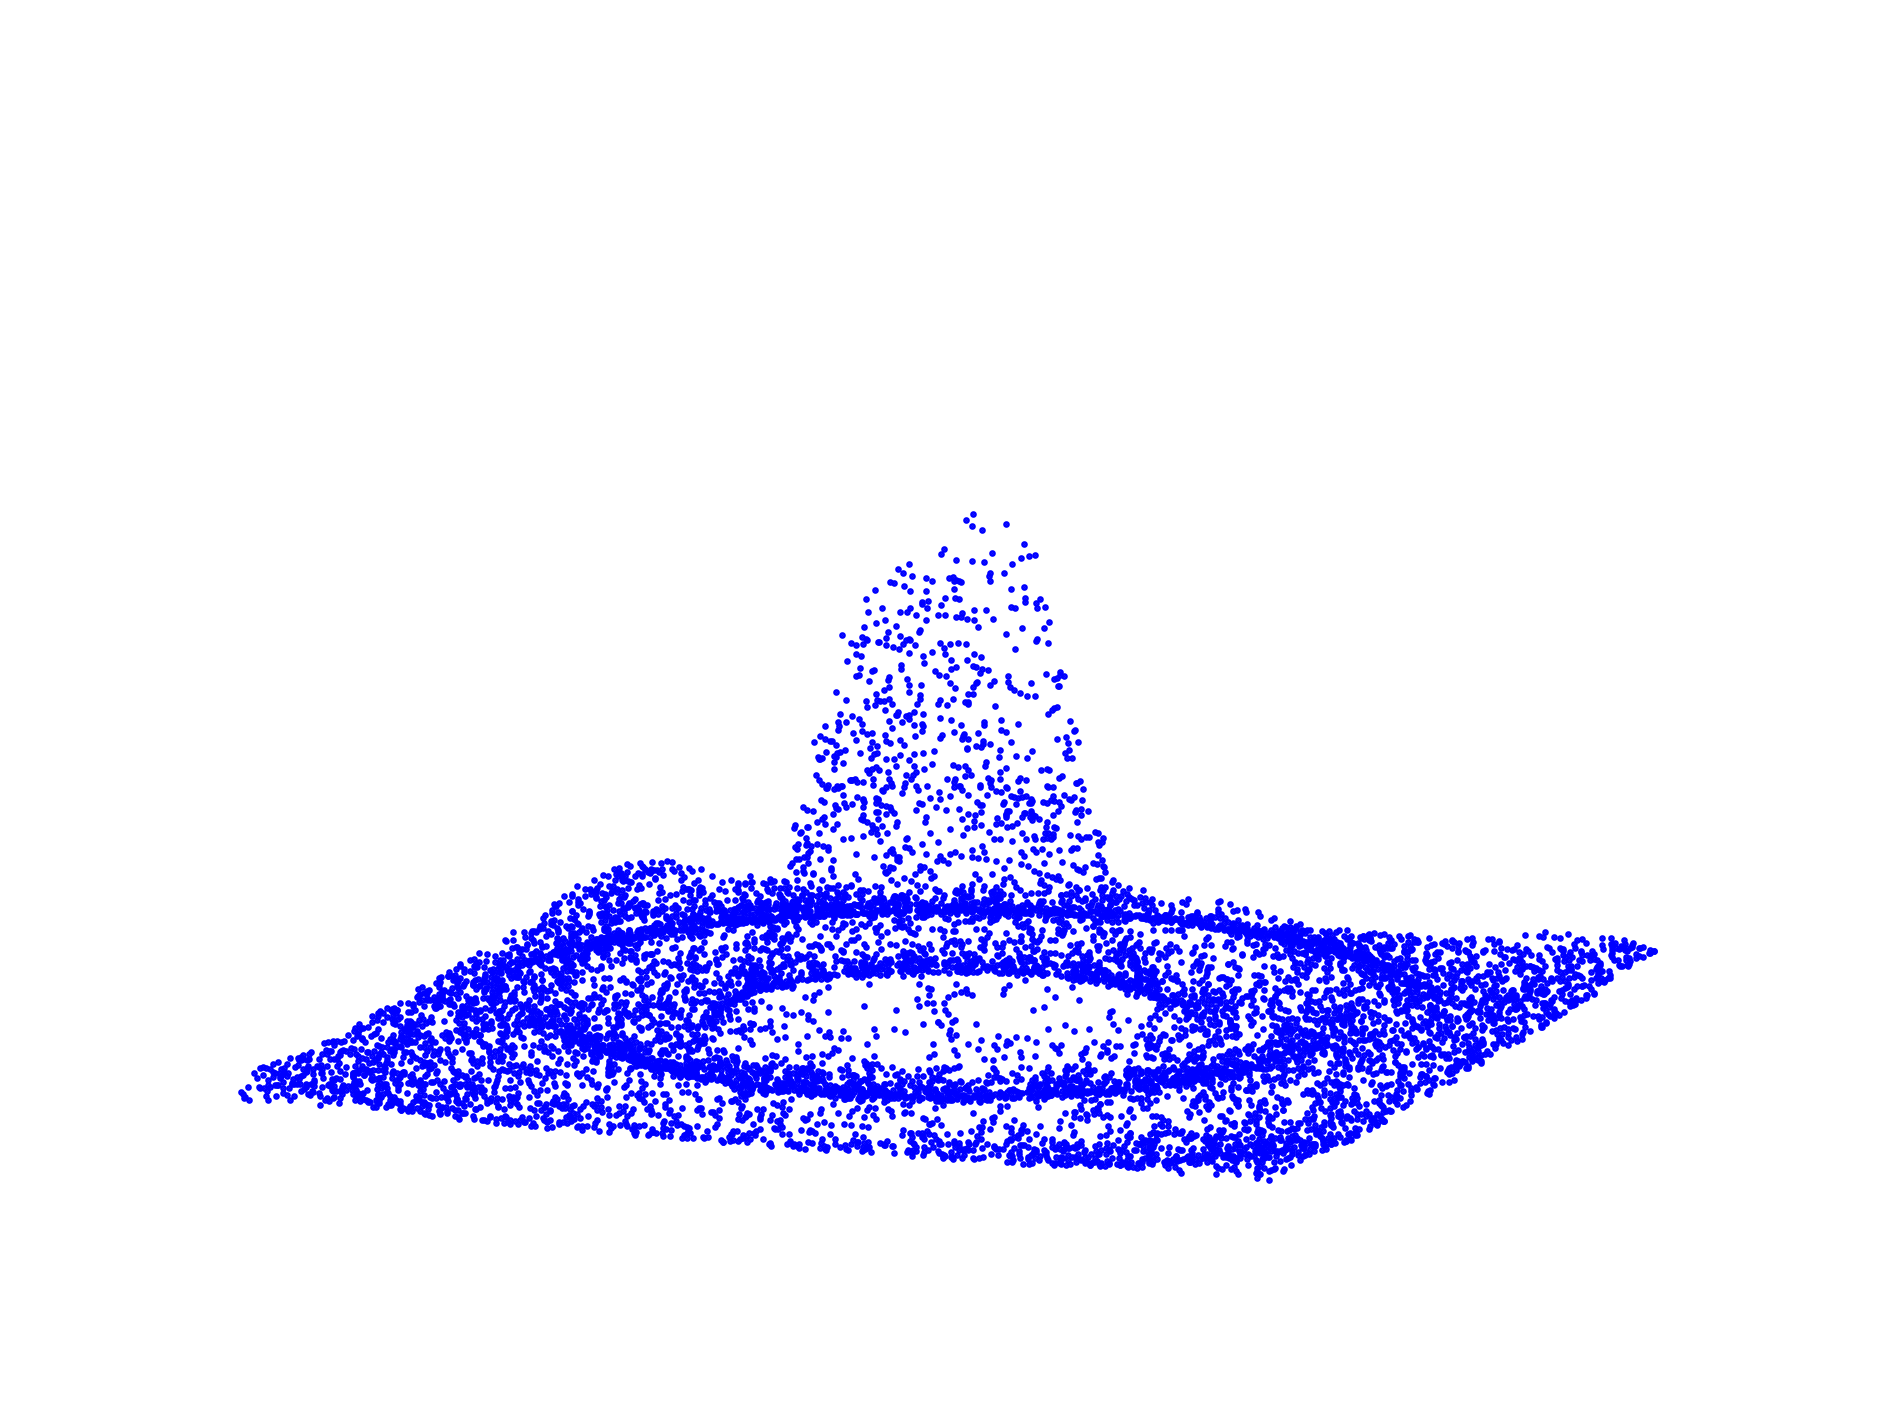
\includegraphics[width=1.\textwidth]{img/distrib_120.png}
    \subcaption{t = 120 }
\end{subfigure}%
\begin{subfigure}{0.33\textwidth}
    \centering
    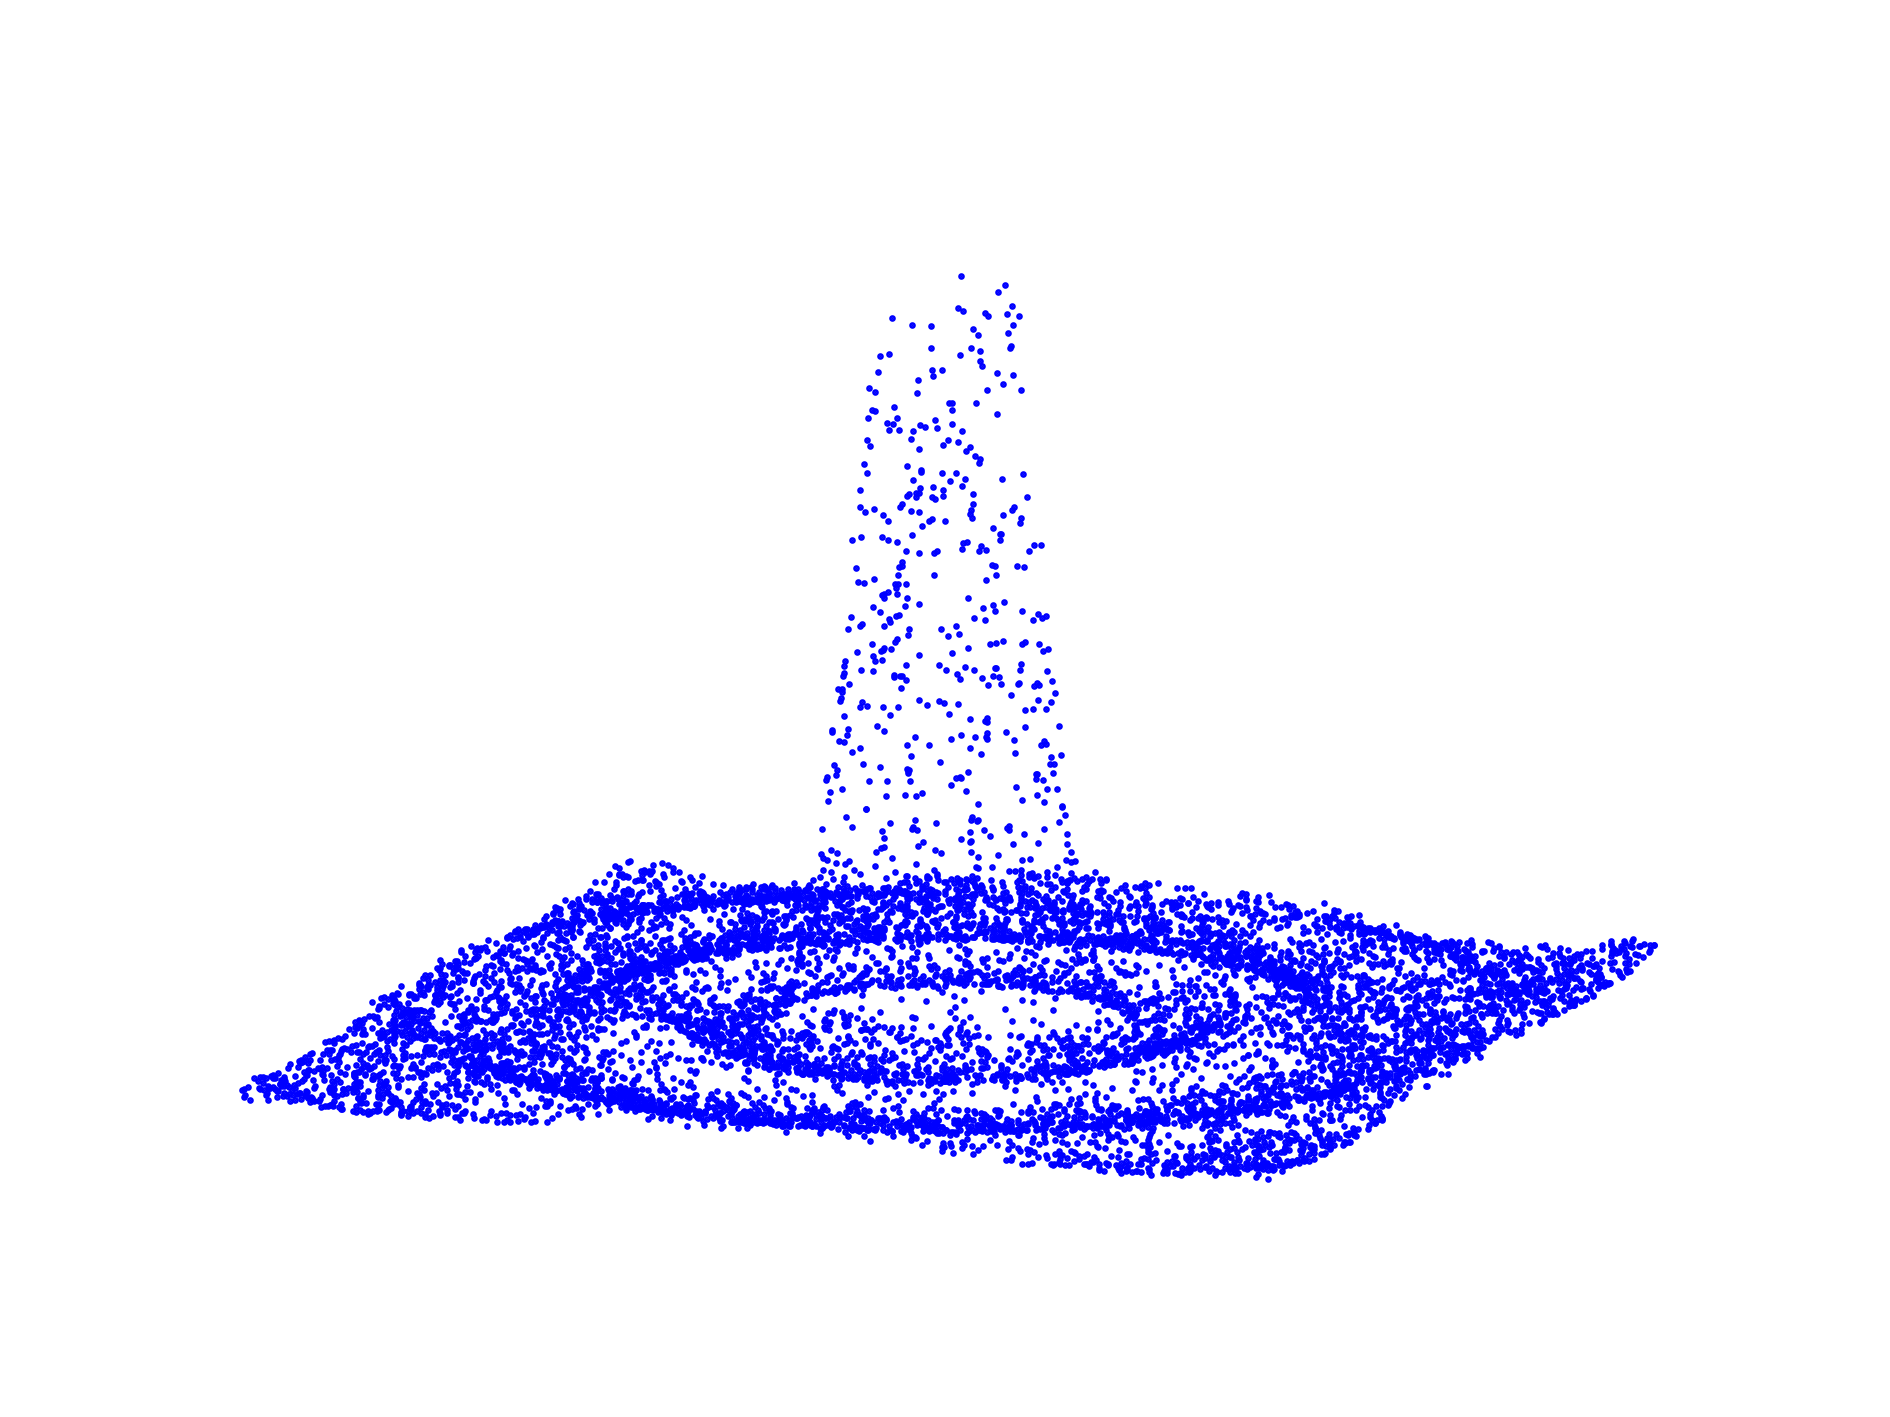
\includegraphics[width=1.\textwidth]{img/distrib_160.png}
    \subcaption{t = 160 }
\end{subfigure}
\caption[short]{Posizioni delle particelle e Energia Cinetica in tre diversi istanti}
\end{figure}


\section{Conclusioni}
Abbiamo considerato tre diversi esempi di particelle in campi elettrici e magnetici, in particolare per l'ultimo caso la simulazione numerica ci ha permesso di comprendere la dinamica non banale del sistema.

\newpage
\definecolor{mygreen}{rgb}{0,0.6,0}
\definecolor{mygray}{rgb}{0.5,0.5,0.5}
\definecolor{mymauve}{rgb}{0.58,0,0.82}
\lstset{
  commentstyle=\color{mygreen},    % comment style
  frame=single,	                   % adds a frame around the code
  keepspaces=true,                 % keeps spaces in text, useful for keeping indentation of code (possibly needs columns=flexible)
  keywordstyle=\color{blue},       % keyword style  
  stringstyle=\color{mymauve},     % string literal style
  showstringspaces=false}


\begin{appendices}
\subsection{Boris Pusher Algorithm}\label{boris}
Uno step di integrazione da $x^n$ e $ v^{n} $ a $x^{n+1}$ e $v^{n+1}$:

$$\mathbf{x}^{n+\frac{1}{2}} = x^{n} + \frac{1}{2}\Delta_t \mathbf{v}^n  \qquad \qquad (drift)$$
$$\mathbf{v}^- = \mathbf{v}^n + \frac{1}{2}\mathbf{E}^{n + \frac{1}{2}}\qquad \qquad (kick)$$
$$\mathbf{v}^+ = \mathbf{v}^- + 2\frac{\mathbf{v}^- + \mathbf{v}^- \times \mathbf{b}}{1 + \mathbf{b}^2} \times  \mathbf{b}\quad  (rotate)$$
$$ \mathbf{v}^{n+1} = \mathbf{v}^+ + \frac{1}{2} \mathbf{E}^{n + \frac{1}{2}}\qquad \qquad (kick)$$
$$ \mathbf{x}^{n+1} = \mathbf{x}^{n+\frac{1}{2}} + \frac{1}{2}\Delta_t \mathbf{v}^{n+1}\qquad \qquad (drift)$$


\subsection{Implementazione singola particella}
\lstinputlisting[language=C++]{../caso1/case1_new.cpp}


\subsection{Implementazione ExB Drift}
\lstinputlisting[language=C++]{../caso2/case2.cpp}


\subsection{Implementazione 10k particelle}
\lstinputlisting[language=C++]{../caso3/borismod.cpp}


\end{appendices}
\end{document}
